\documentclass[12pt,letterpaper]{article}

\usepackage{amsmath, amsthm}
\usepackage{microtype, parskip}
\usepackage[comma,numbers,sort&compress]{natbib}
\usepackage{lineno}
\usepackage{docmute}
\usepackage{caption, subcaption, multirow, morefloats, rotating}
\usepackage{wrapfig}

\frenchspacing

\begin{document}

\section*{Results}

The posterior estimates and analysis in this study take one of two forms: direct inspection of parameter estimates from both models, and downstream estimates of diversity and diversification rates based on posterior predictive simulations from the birth-death model as explained below in the comparison of the models' posterior predictive check results.

\subsection*{Comparing parameter estimates from the pure-presence and birth-death models}

% look at the posterior predictive checks
%   which model has better fit
%   what does that mean?

Comparison of the posterior predictive results from the pure-presence and birth-death models reveals a striking difference in the ability for the model to preidct the structure of the underlying data (Fig. \ref{fig:ppc}). The simulated datasets generated from the birth-death model are clearly able to better reproduce the observed average number of occurrence than the pure-birth model which greatly underestimates the ovserved average number of occurrences. This result means that inferences based on the birth-death model are more likely to be representative of the underlying data than inferences based on the pure-presence model. Further inspection of the posterior parameter estimates from both models can provide further insight into the resons for this difference in posterior predictive results \citep{Gelman2013d}. 

\begin{figure}[ht]
  \begin{subfigure}[b]{0.45\textwidth}
    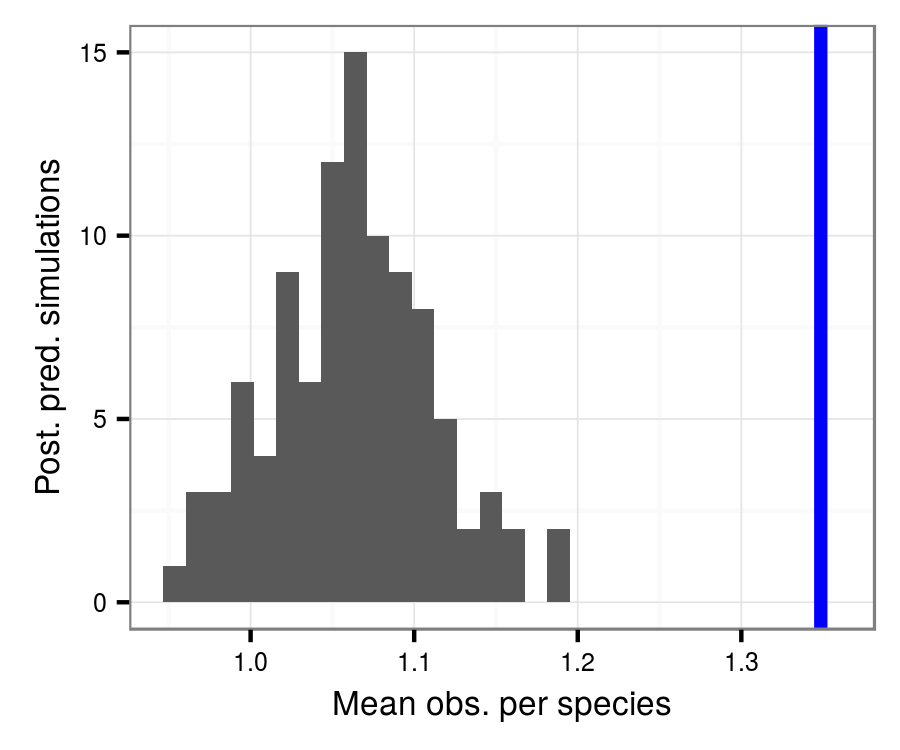
\includegraphics[width=\textwidth,height=0.4\textheight,keepaspectratio=true]{figure/pred_occ}
    \caption{Pure-presence model}
    \label{fig:ppc_pure_presence}
  \end{subfigure}
  \begin{subfigure}[b]{0.45\textwidth}
    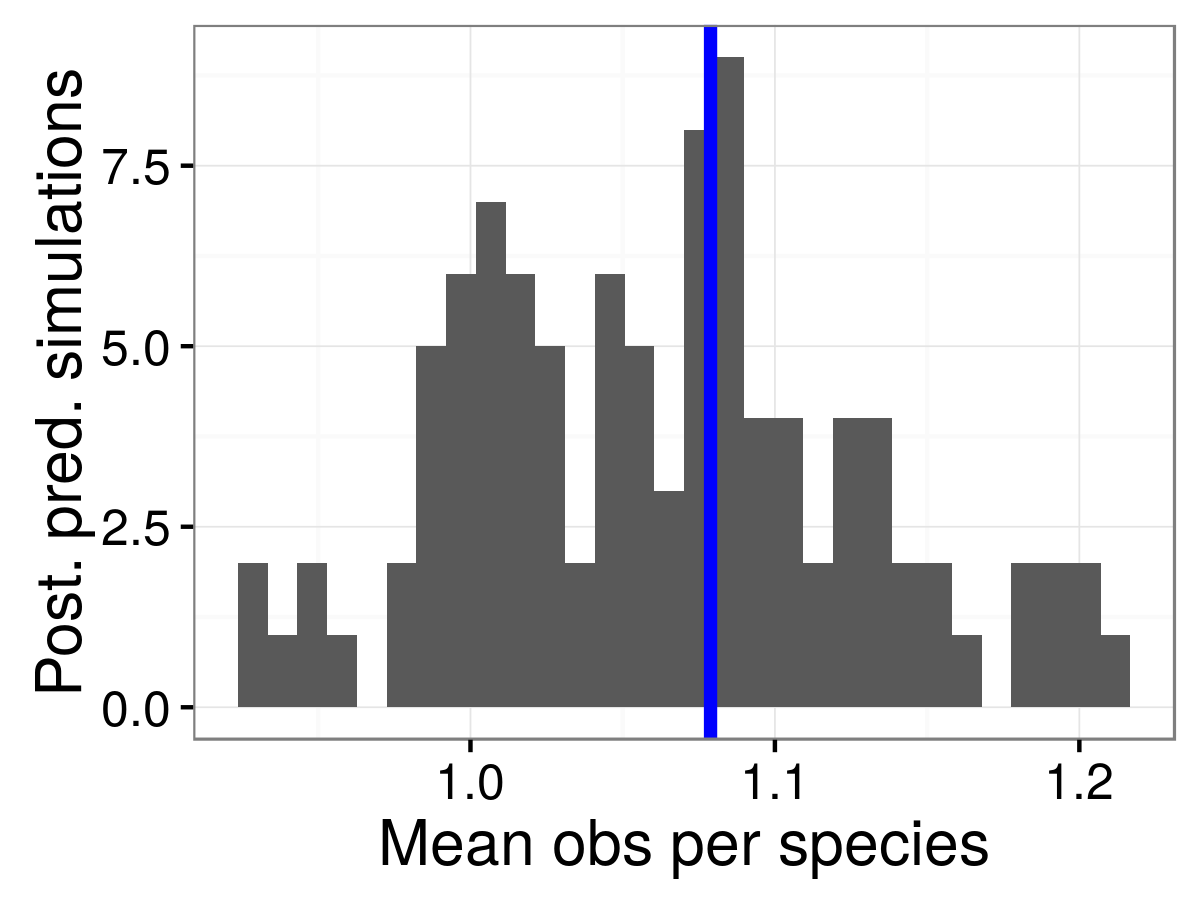
\includegraphics[width=\textwidth,height=0.4\textheight,keepaspectratio=true]{figure/pred_occ_bd}
    \caption{Birth-death model}
    \label{fig:ppc_birth_death}
  \end{subfigure}
  \caption[Posterior predictive check of average occurrence]{Comparison of the average observed number of occurrences per species (blue line) to the average number of occurrences from 100 posterior predictive datasets using the posterior estimates from the pure-presence and birth-death models.}
  \label{fig:ppc}
\end{figure}


Occurrence probabilities estimated from the pure-presence model (Fig. \ref{fig:eco_occur}) are broadly similar to the estimates of origination probability from the birth-death model (Fig. \ref{fig:eco_origin}) as opposed to the estimates of survival probability (Fig. \ref{fig:eco_survival}). This result supports the idea that changes to the North American regional species pool is more likely due to changes to origination than extinction, a result that is returned to later in the discussion of per-capita diversification, origination, and extinction rates.

For most ecotypes, both estimated occurrence probabilities from the pure-presence model (Fig. \ref{fig:eco_occur}) and origination probabilities estimated from the birth-death model (Fig. \ref{fig:eco_origin}) increase with time. This makes sense given that, over time, all species that have at least one observed occurrence must have had that occurrence by the last time point, so our certainty in a species occurring must increase with time. Notably, ecotypes with arboreal components do not appear to follow a similar pattern; instead, occurrence and origination probabilities appear relatively flat for most of the Cenozoic.

The dramatic differences in the estimates origination and survival probabilities are indicative of how differently these processes affect the diversification process and may also be responsible for the better posterior predictive perfomance of the birth-death model over the pure-presence model (Fig. \ref{fig:ppc_pure_presence}, and \ref{fig:ppc_birth_death}). While the estimates at all points along both time series have high variance, what is striking is how mean origination probability changes over time while most ecotype survival probabilities have relatively stable means for the entire Cenozoic (Fig. \ref{fig:eco_origin}, and \ref{fig:eco_survival}).

For most ecotypes, the estimates of origination probabilities are with less uncertainty than similar estimates of survival probabilities (Fig. \ref{fig:eco_origin}, and \ref{fig:eco_survival}). In logistic regression, high uncertainty in the estimates of the underlying log-odds of occurrence, origination, or survival tends to be indicative of extreme rarity or complete absence of the specific ecotype; the latter is called complete separation which occurs when there is no uncertainty in the effect of a covariate on presence/absence, the effect of which has been mitigated by the hierarchical modeling strategy used here \citep{Gelman2013d,Gelman2007} CITATION Statistical Rethinking.


\begin{figure}[ht]
  \centering
  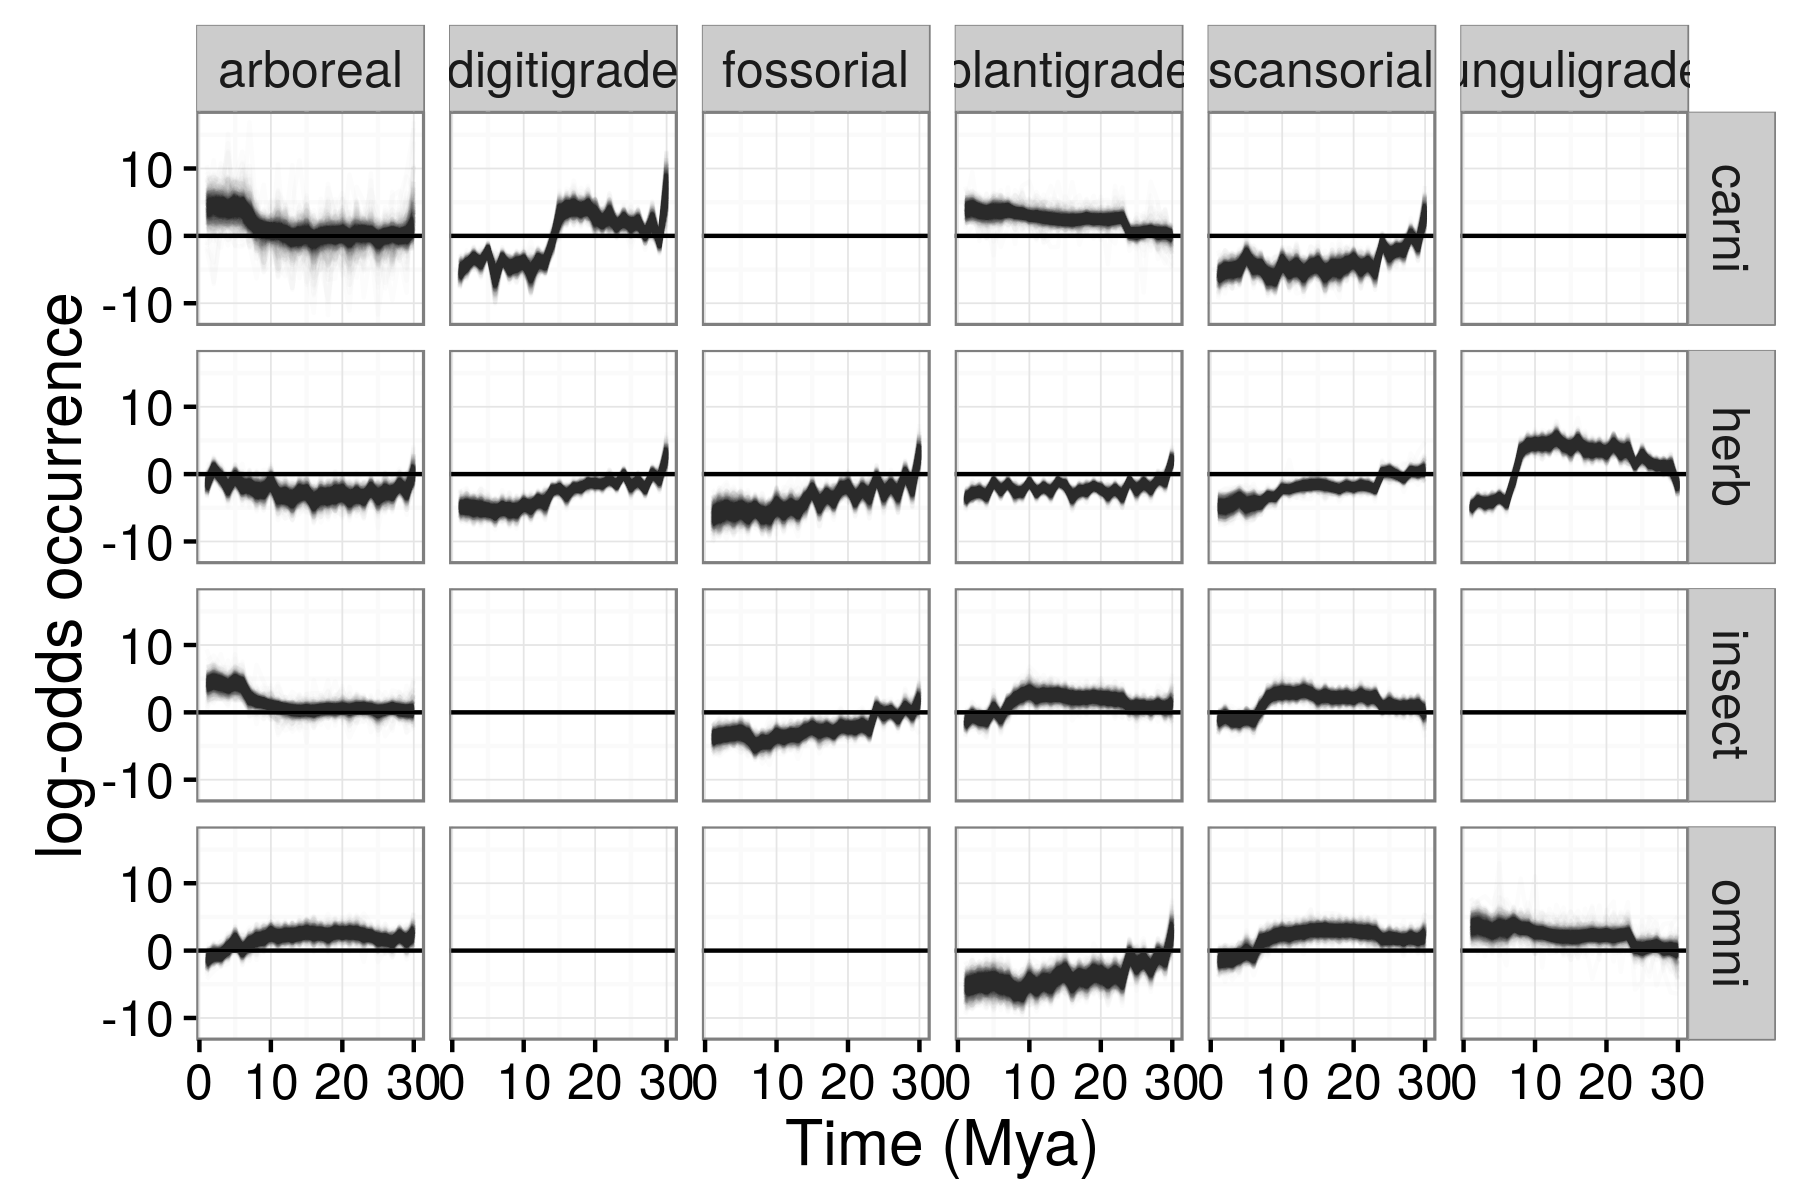
\includegraphics[width=\textwidth,height=0.5\textheight,keepaspectratio=true]{figure/ecotype_occurrence}
  \caption[Ecotype occurrence probability estimated from the pure-presence model]{Probability of a mammal ecotype occurring over time as estimated from the pure-presence model. Each panel depicts 100 random samples from the model's posterior. The columns are by locomotor category and rows by dietary category; their intersections are the observed and analyzed ecotypes. Panels with no lines are ecotypes not observed in the dataset.}
  \label{fig:eco_occur}
\end{figure}

\begin{figure}[ht]
  \centering
  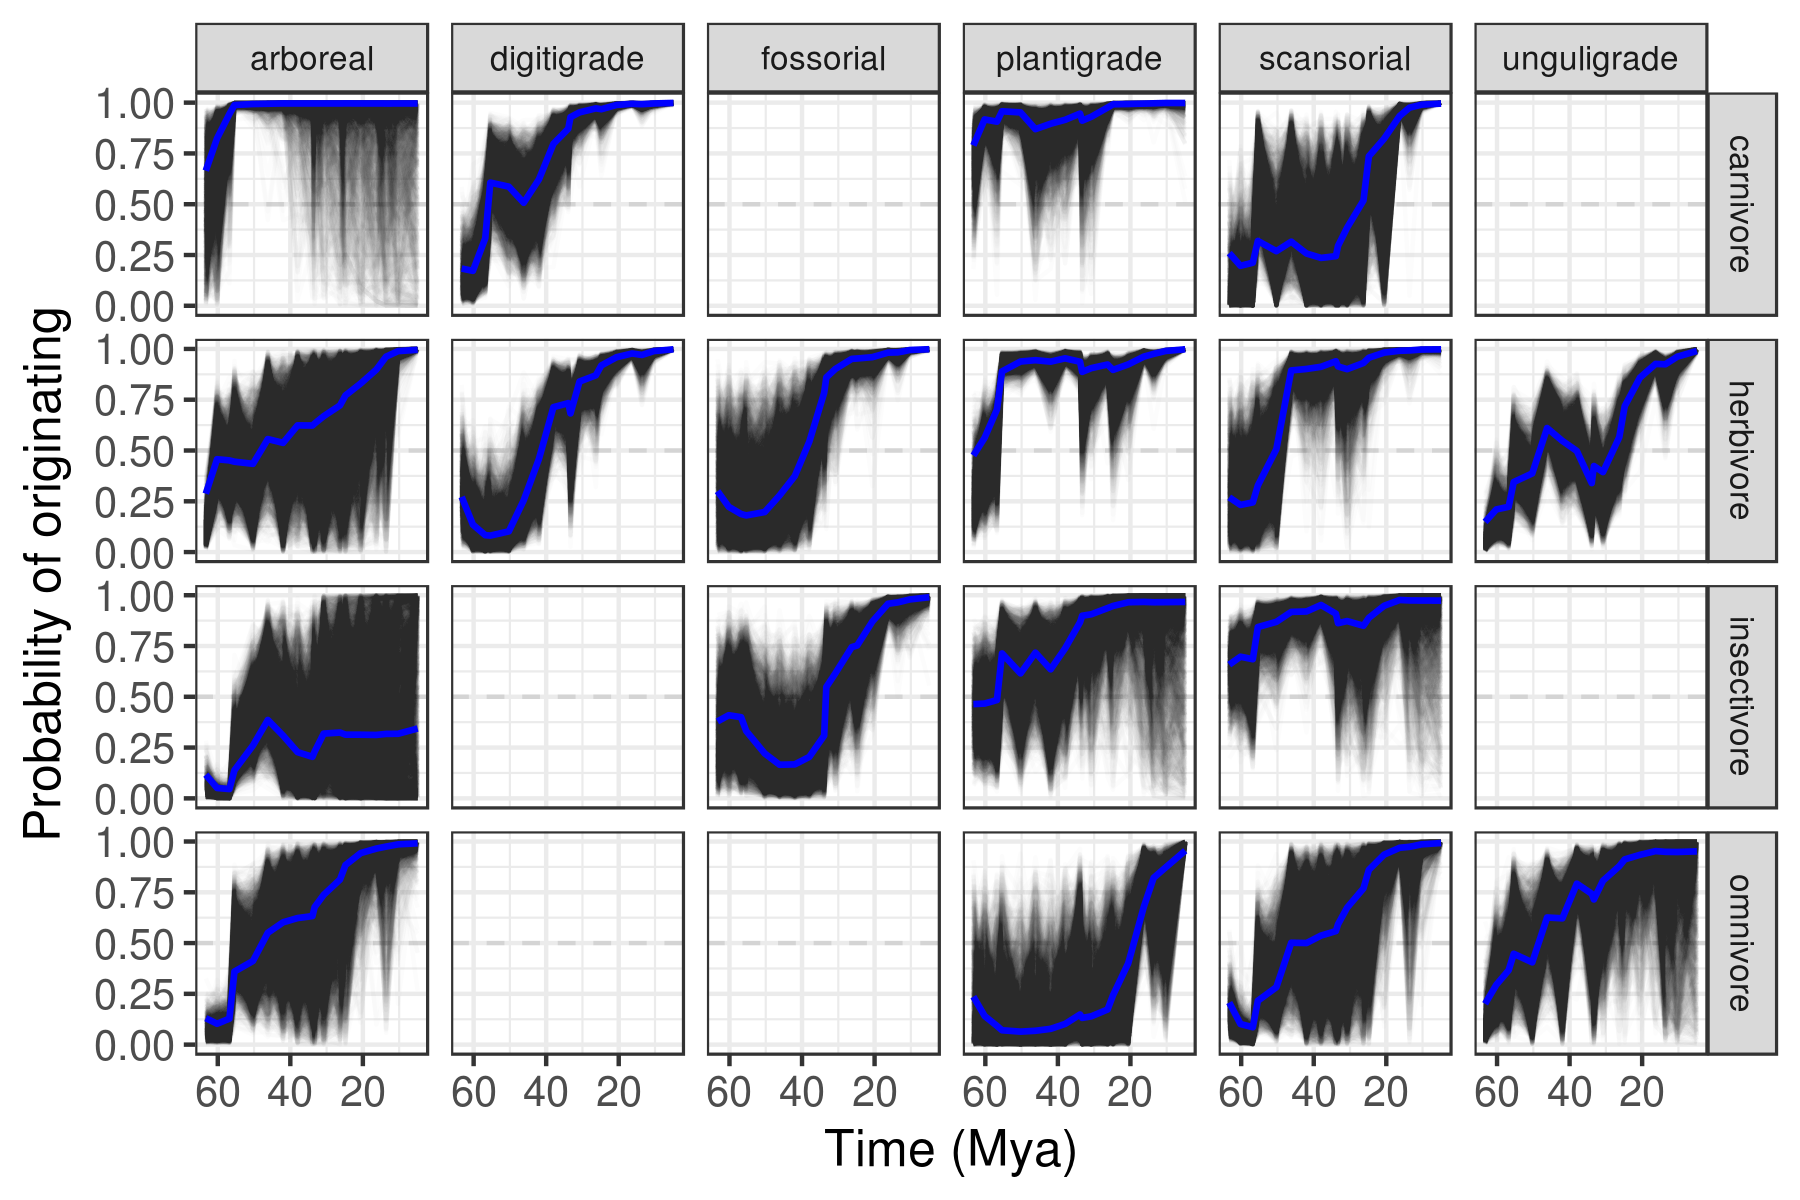
\includegraphics[width=\textwidth,height=0.5\textheight,keepaspectratio=true]{figure/ecotype_origin_bd}
  \caption[Ecotype origination probability estimated from the birth-death model]{Probability of a mammal ecotype origination probabliities at each time point as estimated from the birth-death model. Each panel depicts 100 random samples from the model's posterior. The columns are by locomotor category and rows by dietary category; their intersections are the observed and analyzed ecotypes. Panels with no lines are ecotypes not observed in the dataset.}
  \label{fig:eco_origin}
\end{figure}

\begin{figure}[ht]
  \centering
  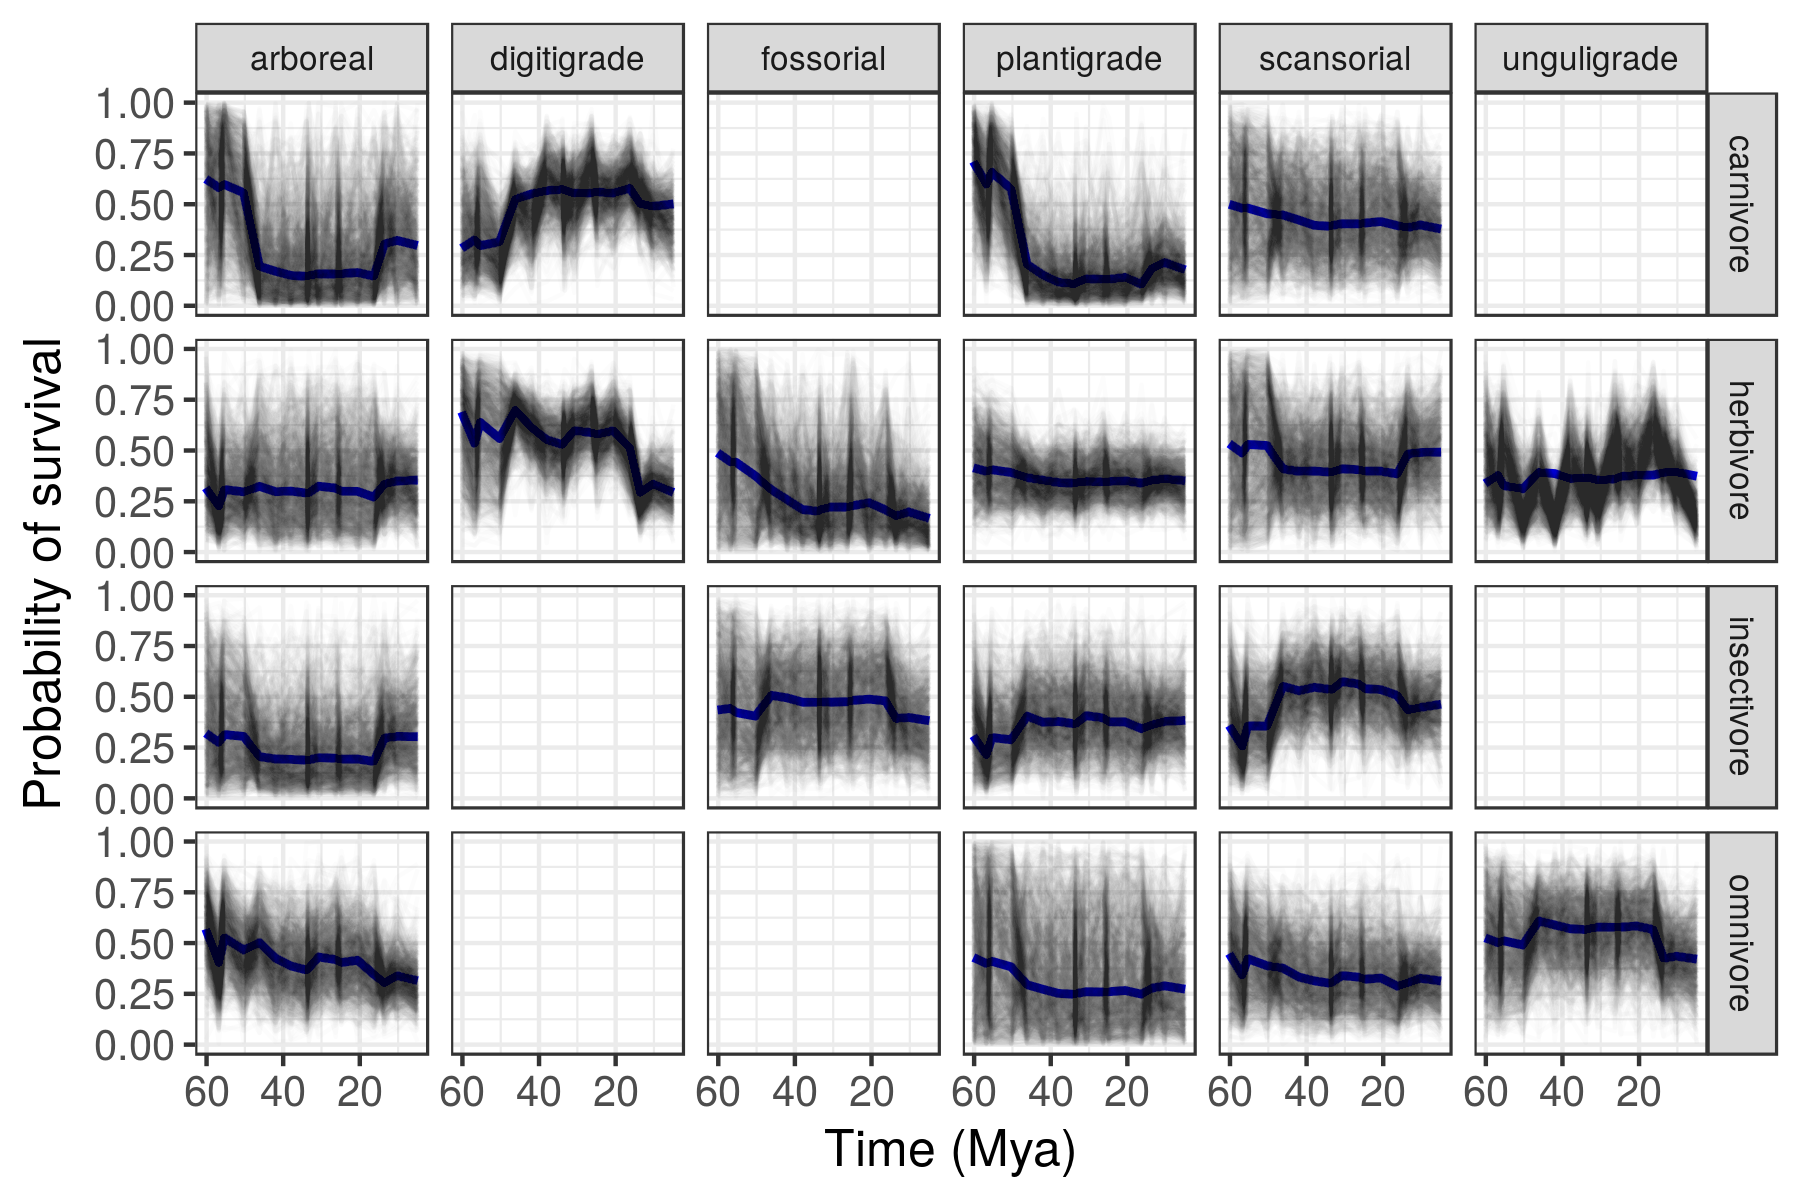
\includegraphics[width=\textwidth,height=0.5\textheight,keepaspectratio=true]{figure/ecotype_survival_bd}
  \caption[Ecotype survival probability estimated from the birth-death model]{Probability of a mammal ecotype survival probabilities at each time point as estimated from the birth-death model. Each panel depicts 100 random samples from the model's posterior. The columns are by locomotor category and rows by dietary category; their intersections are the observed and analyzed ecotypes. Panels with no lines are ecotypes not observed in the dataset.}
  \label{fig:eco_survival}
\end{figure}





The pure-presence and birth-death models also differ in the estimated effect of mass on the probability of sampling a species that is present (Fig. \ref{fig:mass_preserve}). For the pure-presence model, mass is estimated to not have a great effect on the probability of sampling a species that is presence (Fig. \ref{fig:mass_preserve_pure_pres}). Contrastingly, for the birth-death model mass is found to have a negative relationship with observation such that larger species are less likely to be observed if present than smaller species (Fig. \ref{fig:mass_preserve_bd}). 

The result from the birth-death model may be considered unexpected given that it is generally assumed that larger mammals are more likely to have been collected than smaller mammals CITATION. However, collection is not preservation; similarities in preservation rate indicate similarities in how gap-filled species records are. What this result means is that the record of large bodied species is expected on average to have more gaps in sampling and less consistent from time point to time point than smaller bodied species. Additionally, as this is presence/absence data higher preservation and collection in terms of individual specimens at a location or a single temporal horizon does not necessarily translate to high preservation over time.

The average sampling probabilities for both the pure-presence model and birth-death model are both at the point where (rescaled log) mass equals 0; visual comparison indicates that, on average, sampling probability has greater posterior estimate in the pure-presence model than the birth-death model (Fig.\ref{fig:mass_preserve}). The probability that one estimate is different from the other, however, are not directly calculable as they come from different models; what this tells us is how adding more information to the model (i.e. replacing occurrence with origination and extinction) changes parameter estimates in the model.

\begin{figure}[ht]
  \begin{subfigure}[b]{0.45\textwidth}
    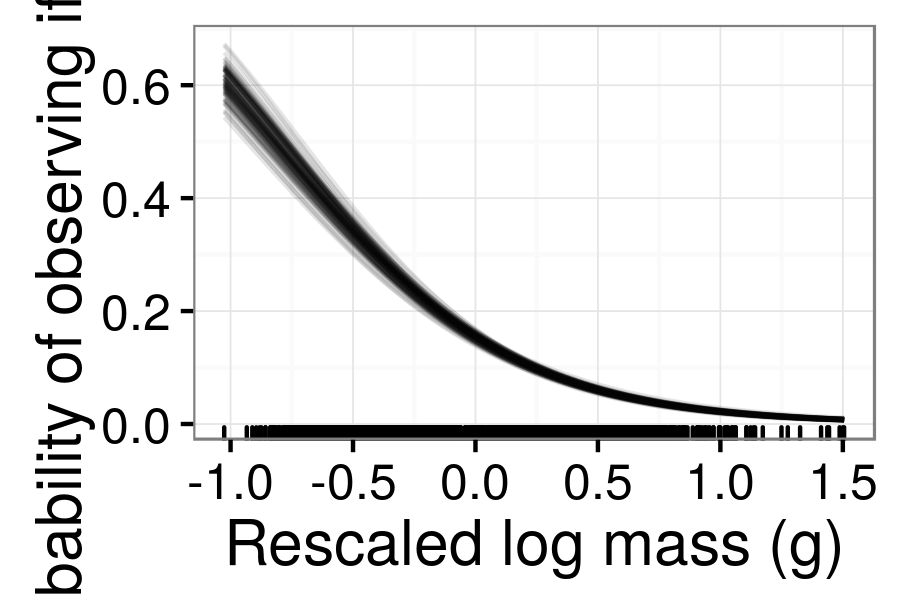
\includegraphics[width=\textwidth,height=0.5\textheight,keepaspectratio=true]{figure/mass_on_samp}
    \caption{Pure-presence model}
    \label{fig:mass_preserve_pure_pres}
  \end{subfigure}
  \begin{subfigure}[b]{0.45\textwidth}
    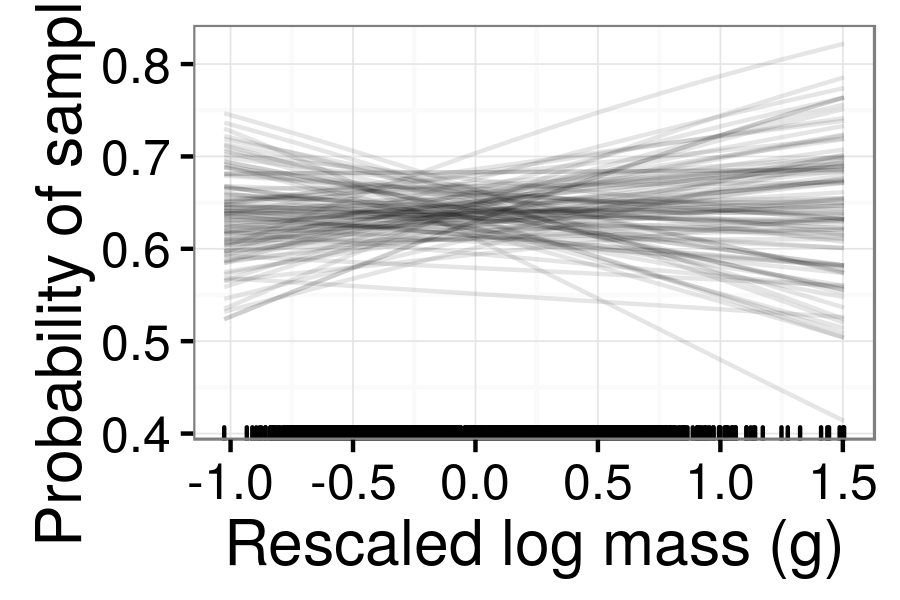
\includegraphics[width=\textwidth,height=0.5\textheight,keepaspectratio=true]{figure/mass_on_samp_bd}
    \caption{Birth-death model}
    \label{fig:mass_preserve_bd}
  \end{subfigure}
  \caption[Estimates of the effect of mass on observation probability]{Estimates of the effect of species mass on probability of sampling a present species (\(p\)). Mass has been log-transformed, centered, and rescaled; this means that a mass of 0 corresponds to the mean of log-mass of all observed species and that mass is in standard deviation units. Estimates are from both the pure-presence and birth-death models.}
  \label{fig:mass_preserve}
\end{figure}


The effect of species mass on probability of occurrence as estimated from the pure-presence (Fig. \ref{fig:mass_occur}) are most similar to the estimated effect of species mass on probability of origination for the birth-death model (Fig. \ref{fig:mass_origin}). The striking pattern observable in both sets of estimates is the higher probability of occurrence for species with body sizes closer to the mean than either extremes. This result is consistent with the canonically normal distribution of mammal body sizes CITATION; it is then expected that the most likely to occur species would be those from the middle of the distribution, and that species originating will on average be of average mass, especially considering species shared common ancestry CITATION. Note that all variation in estimates between ecotypes (Fig. \ref{fig:mass_origin}) is due to differences in ecotype-specific survival probability and the associated effects of plant phase; the effect of mass was considered constant for all ecotypes.

\begin{figure}[ht]
  \centering
  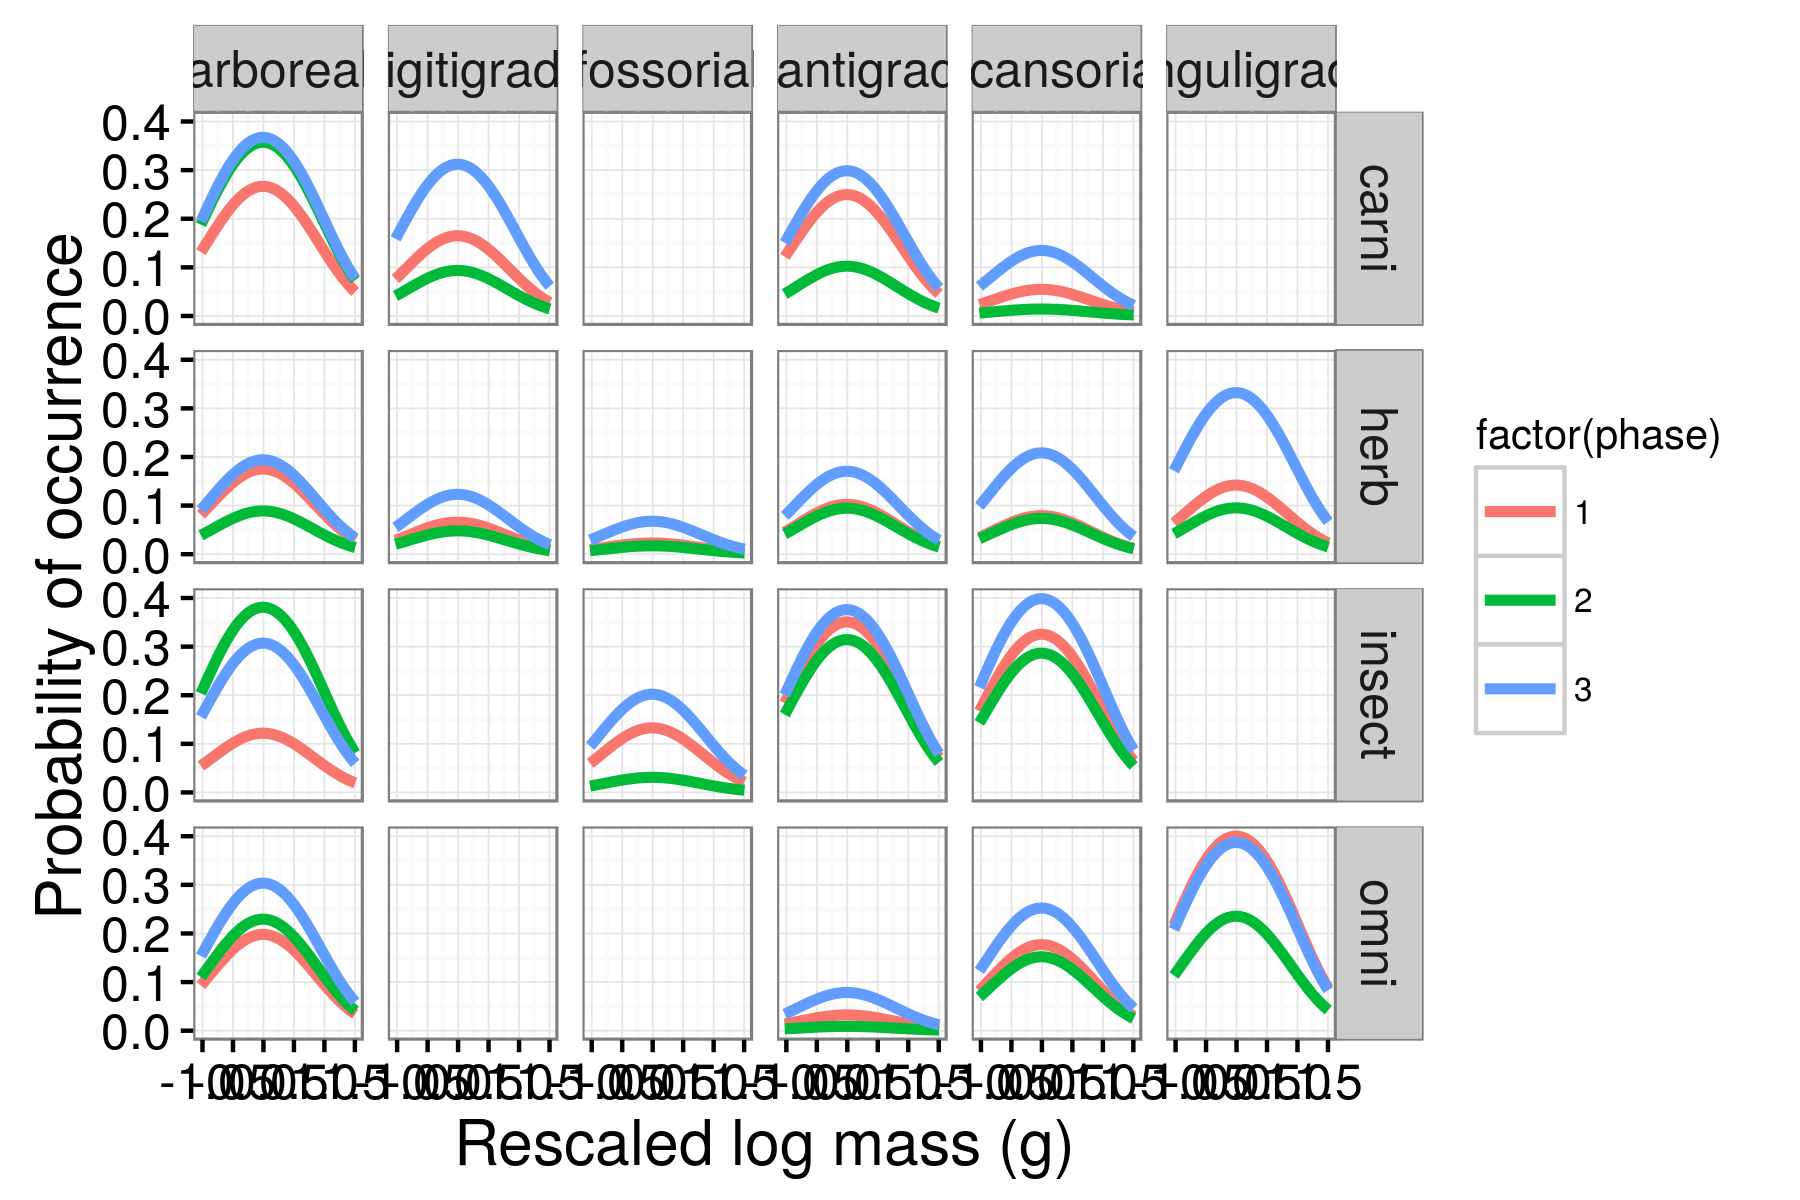
\includegraphics[width=\textwidth,height=0.5\textheight,keepaspectratio=true]{figure/mass_on_pres}
  \caption[Effect of mass on probability of species occurrence as estimated from the pure-presence model]{Mean estimate of the effect of species mass on the probability of a species occurrence for each of the three plant phases. The effect of mass is considered constant over time and that the only aspect of the model that changes with plant phase is the intercept of the relationship between mass and occurrence. The three plant phases are indicated by the color of the line. Mass has been log-transformed, centered, and rescaled; this means that a mass of 0 corresponds to the mean of log-mass of all observed species and that mass is in standard deviation units. Only the mean estimates of the effects of both mass and plant phase are plotted for clarity; these estimates are obviously made with uncertainty.}
  \label{fig:mass_occur}
\end{figure}

\begin{figure}[ht]
  \centering
  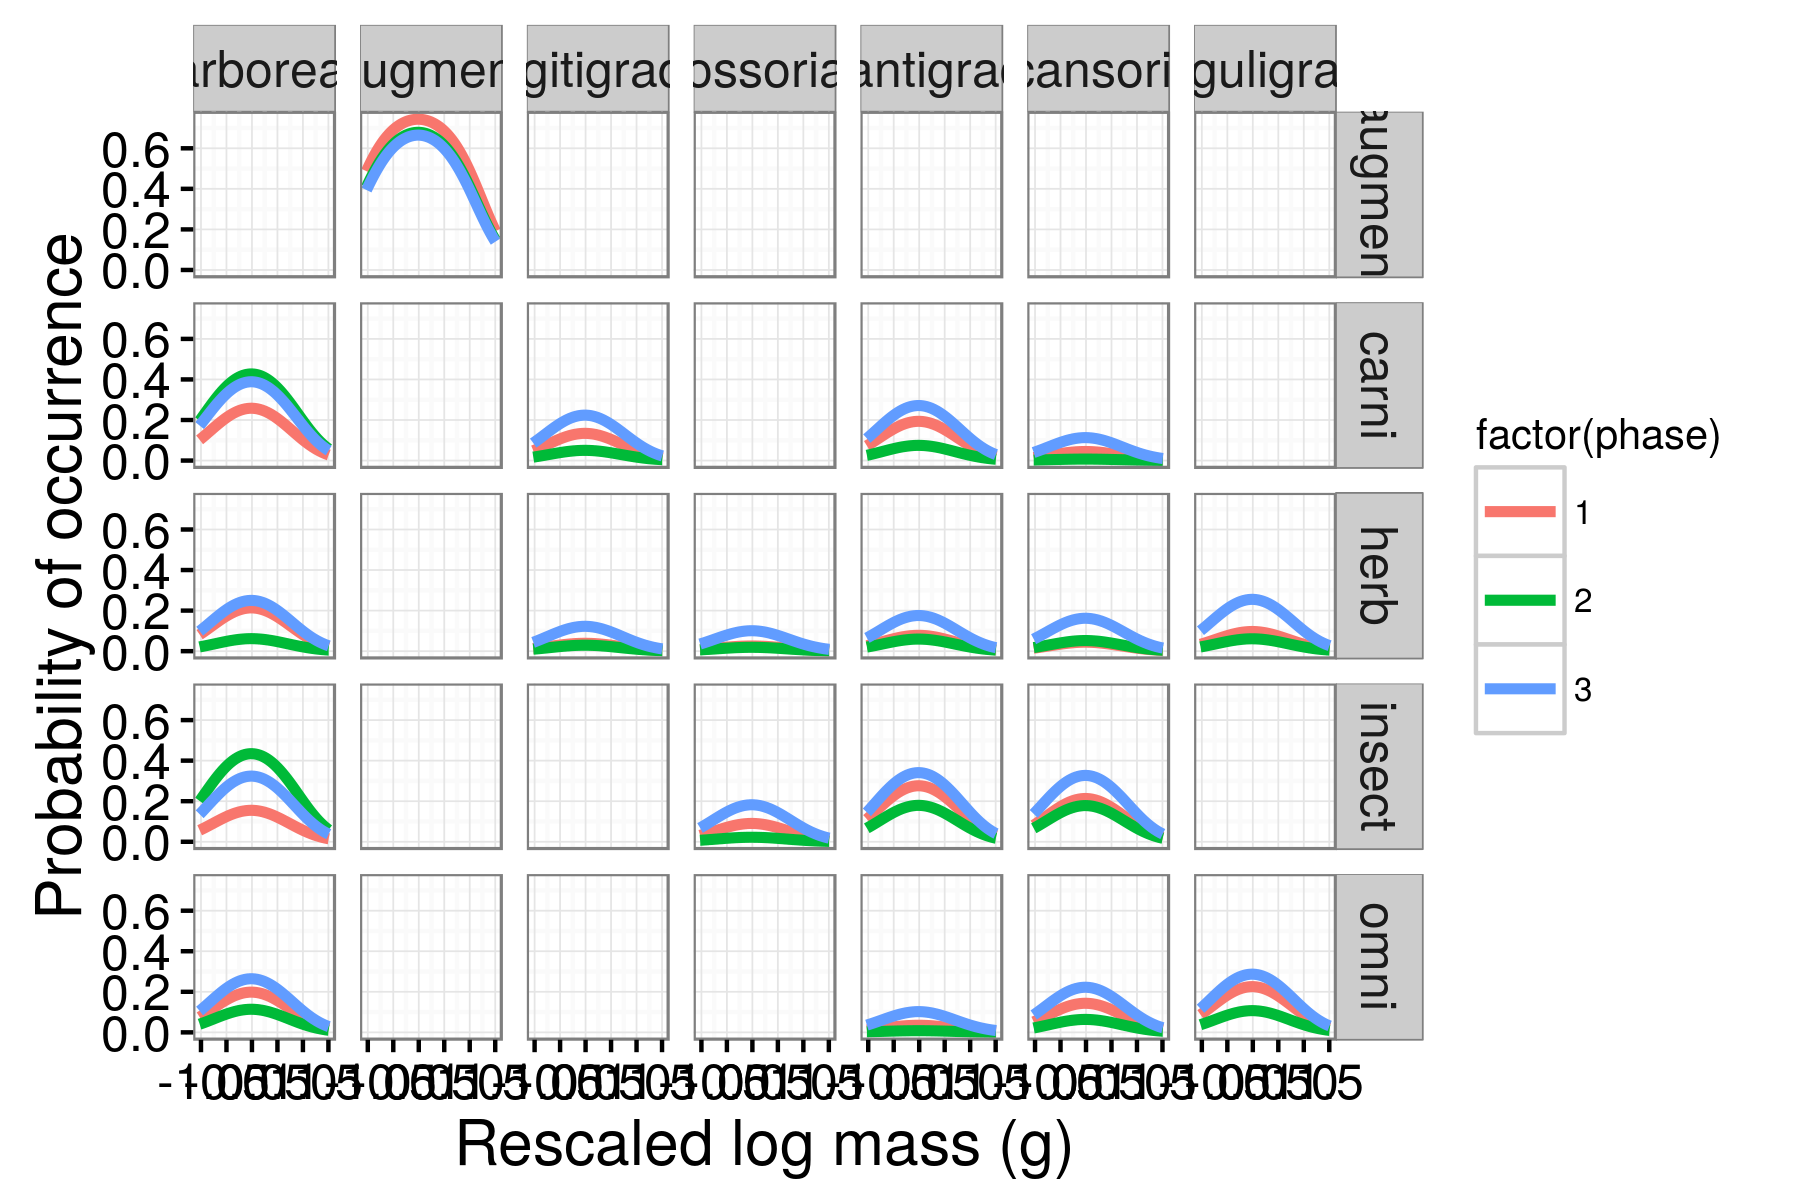
\includegraphics[width=\textwidth,height=0.5\textheight,keepaspectratio=true]{figure/mass_on_origin_bd}
  \caption[Effect of mass on probability of species origination as estimated from the birth-death model]{Mean estimate of the effect of species mass on the probability of a species originating for each of the three plant phases. The effect of mass is considered constant over time and that the only aspect of the model that changes with plant phase is the intercept of the relationship between mass and origination. The three plant phases are indicated by the color of the line. Mass has been log-transformed, centered, and rescaled; this means that a mass of 0 corresponds to the mean of log-mass of all observed species and that mass is in standard deviation units. Only the mean estimates of the effects of both mass and plant phase are plotted for clarity; these estimates are obviously made with uncertainty.}
  \label{fig:mass_origin}
\end{figure}



In contrast, the effect of species mass on probability of survival as estimated from the birth-death model (Fig. \ref{fig:mass_survival}) indicates little effect of mass on extinction; this is consistent with previous findings from the North American mammal fossil record \citep{Smits2015b,Tomiya2013}. Note that all variation between ecotypes (Fig. \ref{fig:mass_survival}) is due to differences in ecotype-specific survival probability and the associated effects of plant phase; the effect of mass was considered constant for all ecotypes.

\begin{figure}[ht]
  \centering
  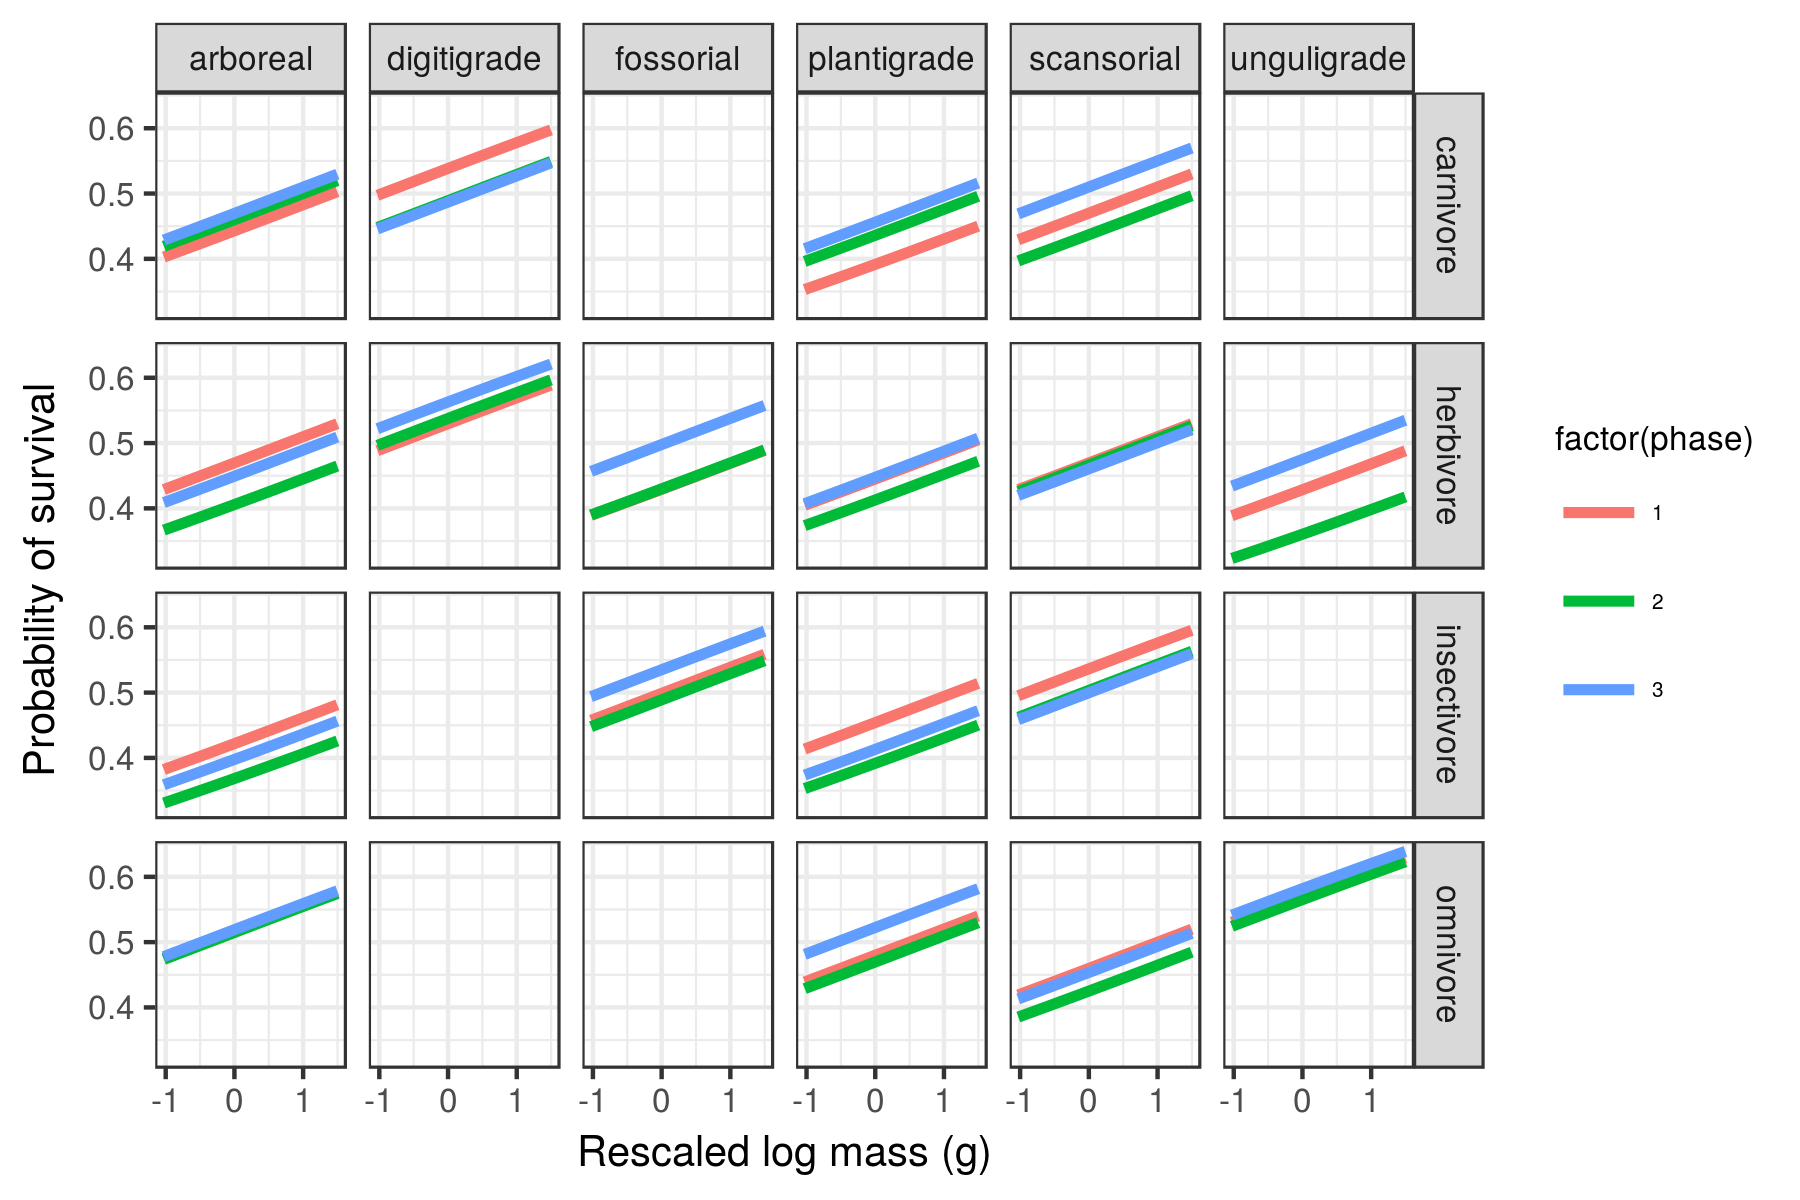
\includegraphics[width=\textwidth,height=0.5\textheight,keepaspectratio=true]{figure/mass_on_surv_bd}
  \caption[Effect of mass on probability of species survival as estimated from the birth-death model]{Mean estimate of the effect of species mass on the probability of a species survival for each of the three plant phases. The effect of mass is considered constant over time and that the only aspect of the model that changes with plant phase is the intercept of the relationship between mass and survival. The three plant phases are indicated by the color of the line. Mass has been log-transformed, centered, and rescaled; this means that a mass of 0 corresponds to the mean of log-mass of all observed species and that mass is in standard deviation units. Only the mean estimates of the effects of both mass and plant plant are plotted for clarity; these estimates are obviously made with uncertainty.}
  \label{fig:mass_survival}
\end{figure}



Similarities in parameters estimates between ecotypes may be due to similar response to environmental factors (Fig. \ref{fig:group_pure_presence}, \ref{fig:group_origin_bd}, and \ref{fig:group_surv_bd}). As with previous comparisons between posterior estimates from the pure-presence and birth-death models, the effects of the group-level covariates in the pure-presence model (Fig. \ref{fig:group_pure_presence})  are more similar to those estimates of the group-level effects on origination (Fig. \ref{fig:group_origin_bd}) as opposed to survival (Fig. \ref{fig:group_surv_bd}). 

As demonstrated in the comparisons of the effect of mass on occurrence from the pure-presence model (Fig. \ref{fig:mass_occur}) with the effect of mass on origination and survival from the birth-death model (Fig. \ref{fig:mass_origin}, and \ref{fig:mass_survival}), there is considerable variation in the effect of plant phases on ecotype-specific estimates.
%occurrence
%  Plant phase
Plant phase is estimated to structure ecotype occurrence probability, specifically at least one phase has a very different estimates from the others, for non-arboreal carnivores, arboreal and unguligrade herbivores, arboreal and fossorial insectivores, and arboreal and unguligrade omnivores (Fig. \ref{fig:group_pure_presence}). For the other ecotypes, plant phase does not correspond to major differences in diversity over time. 
%  Temperature
The temperature covariates do not appear to strongly structure occurrence history for most ecotypes (Fig. \ref{fig:group_pure_presence}). Ecotypes for which at least one temperature covariate is estimated to have strong effect on occurrence are digitigrade canivores (mean only), scansorial carnivores (mean only), and non-arboreal herbivores. For the other ecotypes neither of the global temperature covariates are expected to have strong effects on occurrence history.

  \begin{figure}[ht]
  \centering
  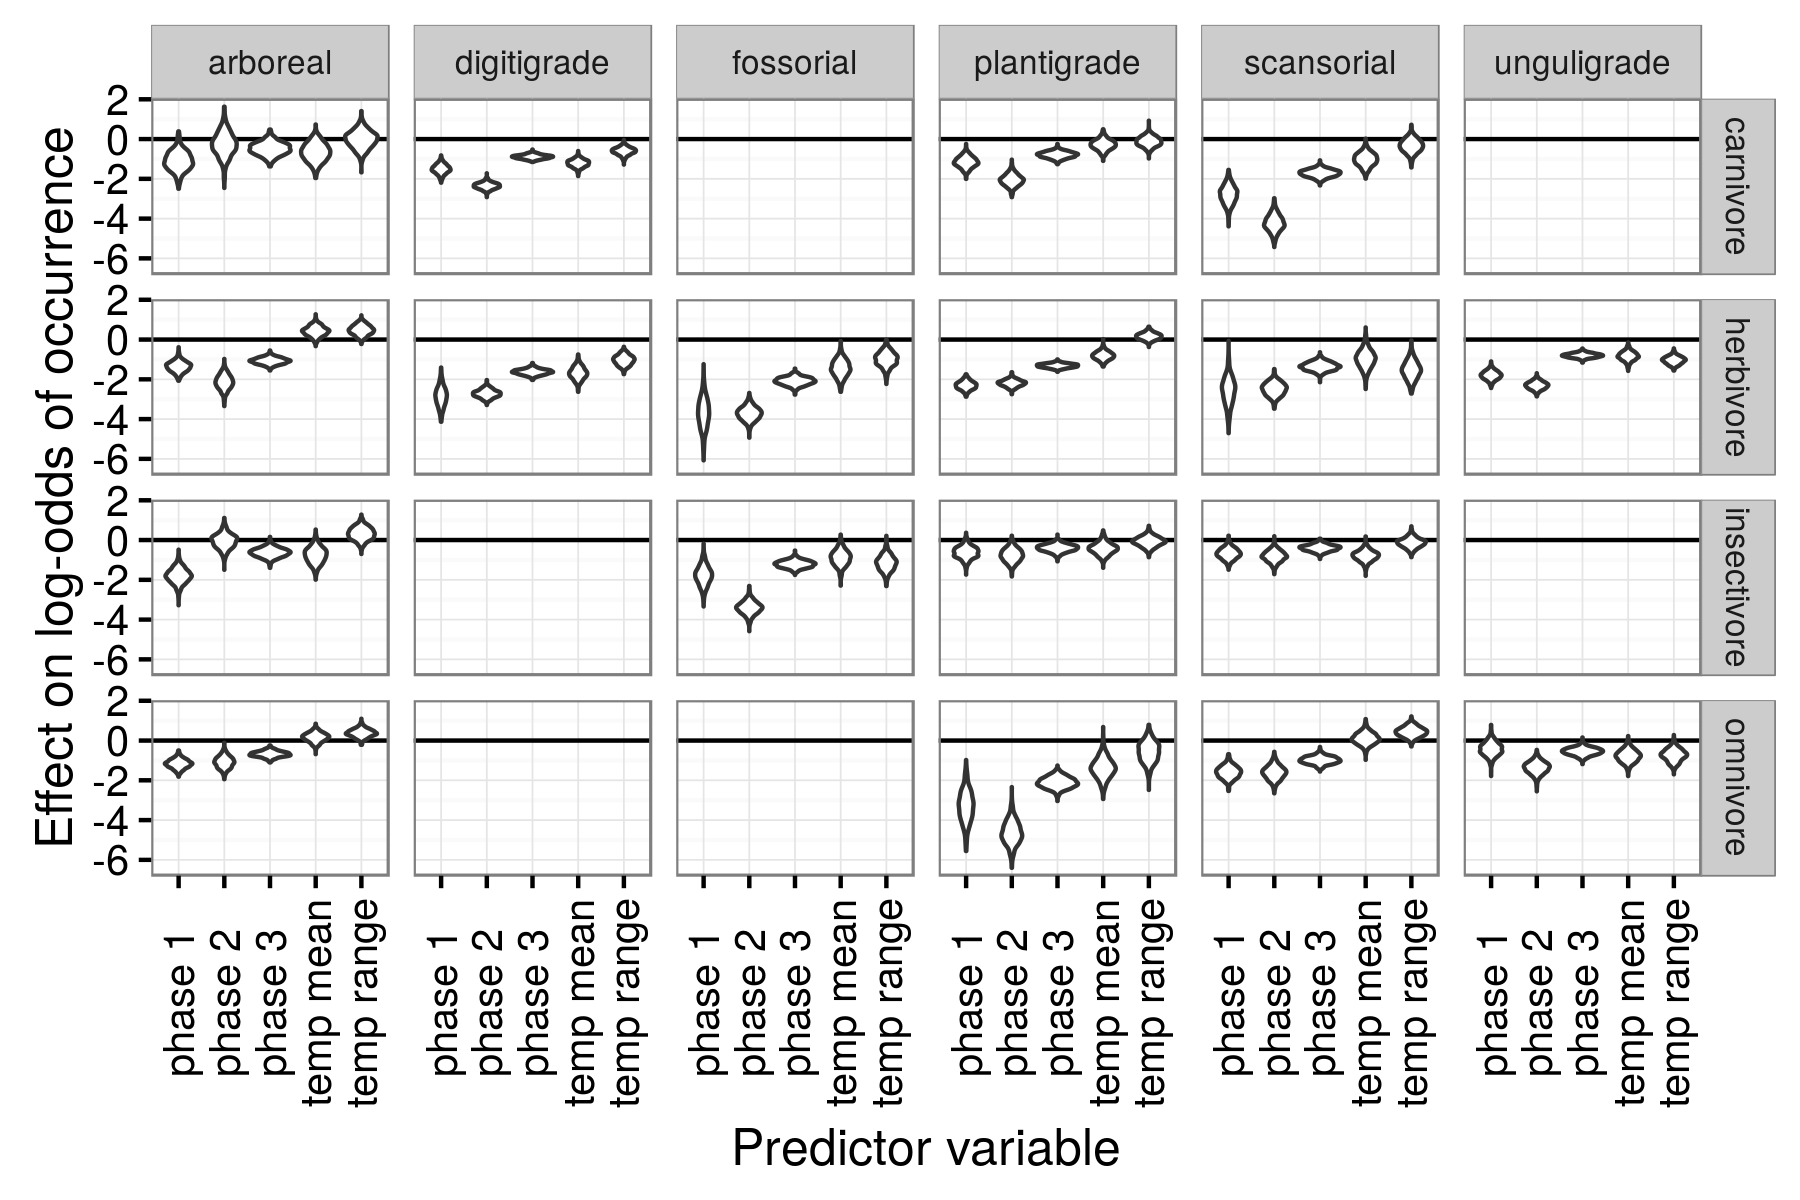
\includegraphics[width=\textwidth,height=0.5\textheight,keepaspectratio=true]{figure/group_on_ecotype}
  \caption[Effects of group-level covariates on log-odds of ecotype occurrence as estimated from the the pure-presence model]{Estimated effects of the group-level covariates describing environmental context on log-odds of species occurrence. These estimates are from the pure-presence model.} 
  \label{fig:group_pure_presence}
\end{figure}



%origination
%  Plant phase
Plant phase is estimated to at least partially structure ecotype origination probability for non-arboreal carnivores, non-fossorial or plantigrade herbivores, arboreal and fossorial insectivores, and plantigrade and scansorial omnivores (Fig. \ref{fig:group_origin_bd}). 
%  Temperature
In the case of the temperature covariates, at least one of them is estimated to have strong effects on origination history for the following ecotypes: digitigrade carnivores, and both digitigrade and unguligrade herbivores (Fig. \ref{fig:group_origin_bd}). Neither of the temperature covariates are estimate to have strong effects for the other ecotypes. Results like these, assuming their accuracy, are probably responsible for many of the arguments over the effects of climate on mammal diversity and diversification \citep{Alroy1996a,Alroy2000g,Figueirido2012,Janis1993c,Blois2009}; because different ecotypes have different responses, a myopic or limited view of mammal diversity can be misleading when attempting to generalize for the entire system.

\begin{figure}[ht]
  \centering
  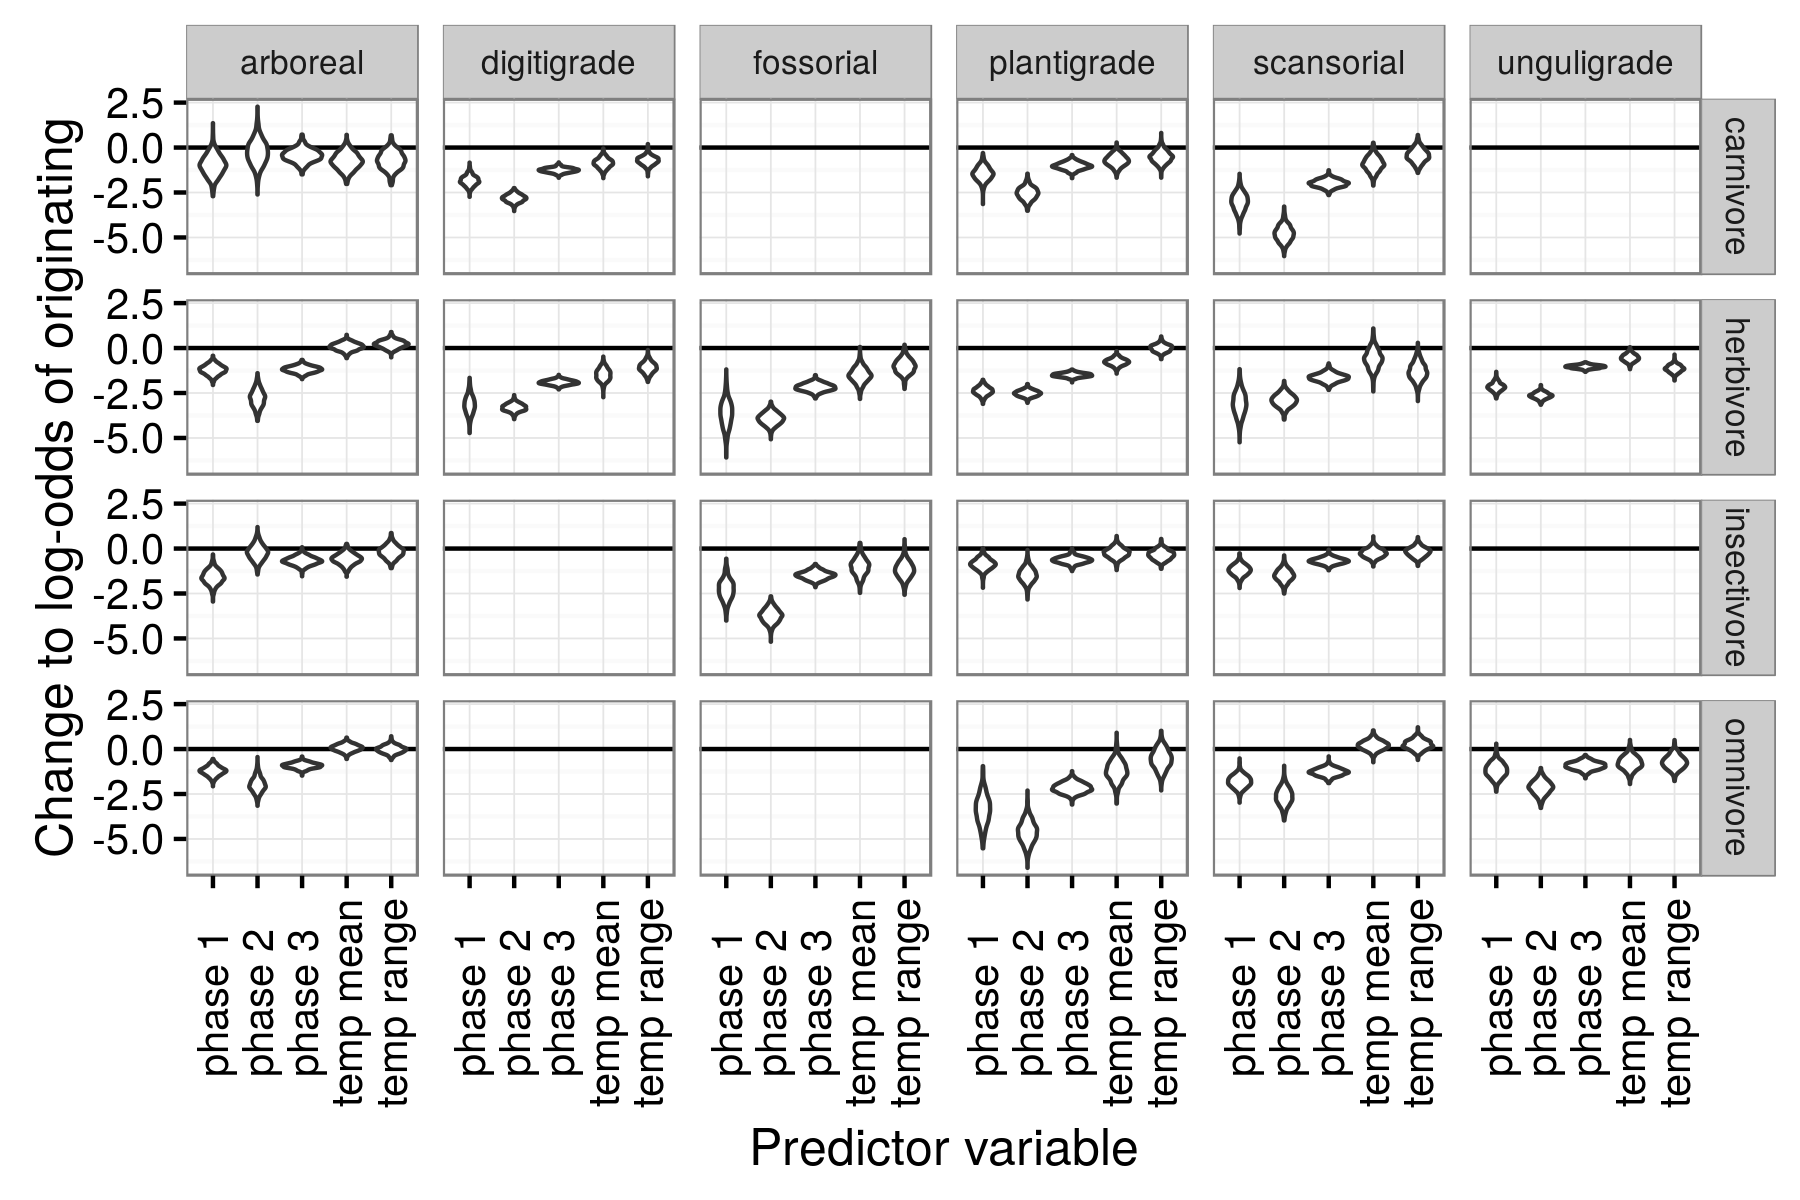
\includegraphics[width=\textwidth,height=0.5\textheight,keepaspectratio=true]{figure/group_on_origin_bd}
  \caption[Effects of group-level covariates on log-odds of ecotype origination as estimated from the the birth-death model]{Estimated effects of the group-level covariates describing environmental context on log-odds of species origination. These estimates are from the birth-death model.}
  \label{fig:group_origin_bd}
\end{figure}


%survival
%  Plant phase
%  Temperature
In contrast to both of the descriptions above of the group-level effects on origination (Fig. \ref{fig:group_pure_presence}, and \ref{fig:group_origin_bd}), group-level covariates are estimate to have almost no effect on survival for all ecotypes (Fig. \ref{fig:group_surv_bd}); this is the case for both the plant phases and temperature covariates.

\begin{figure}[ht]
  \centering
  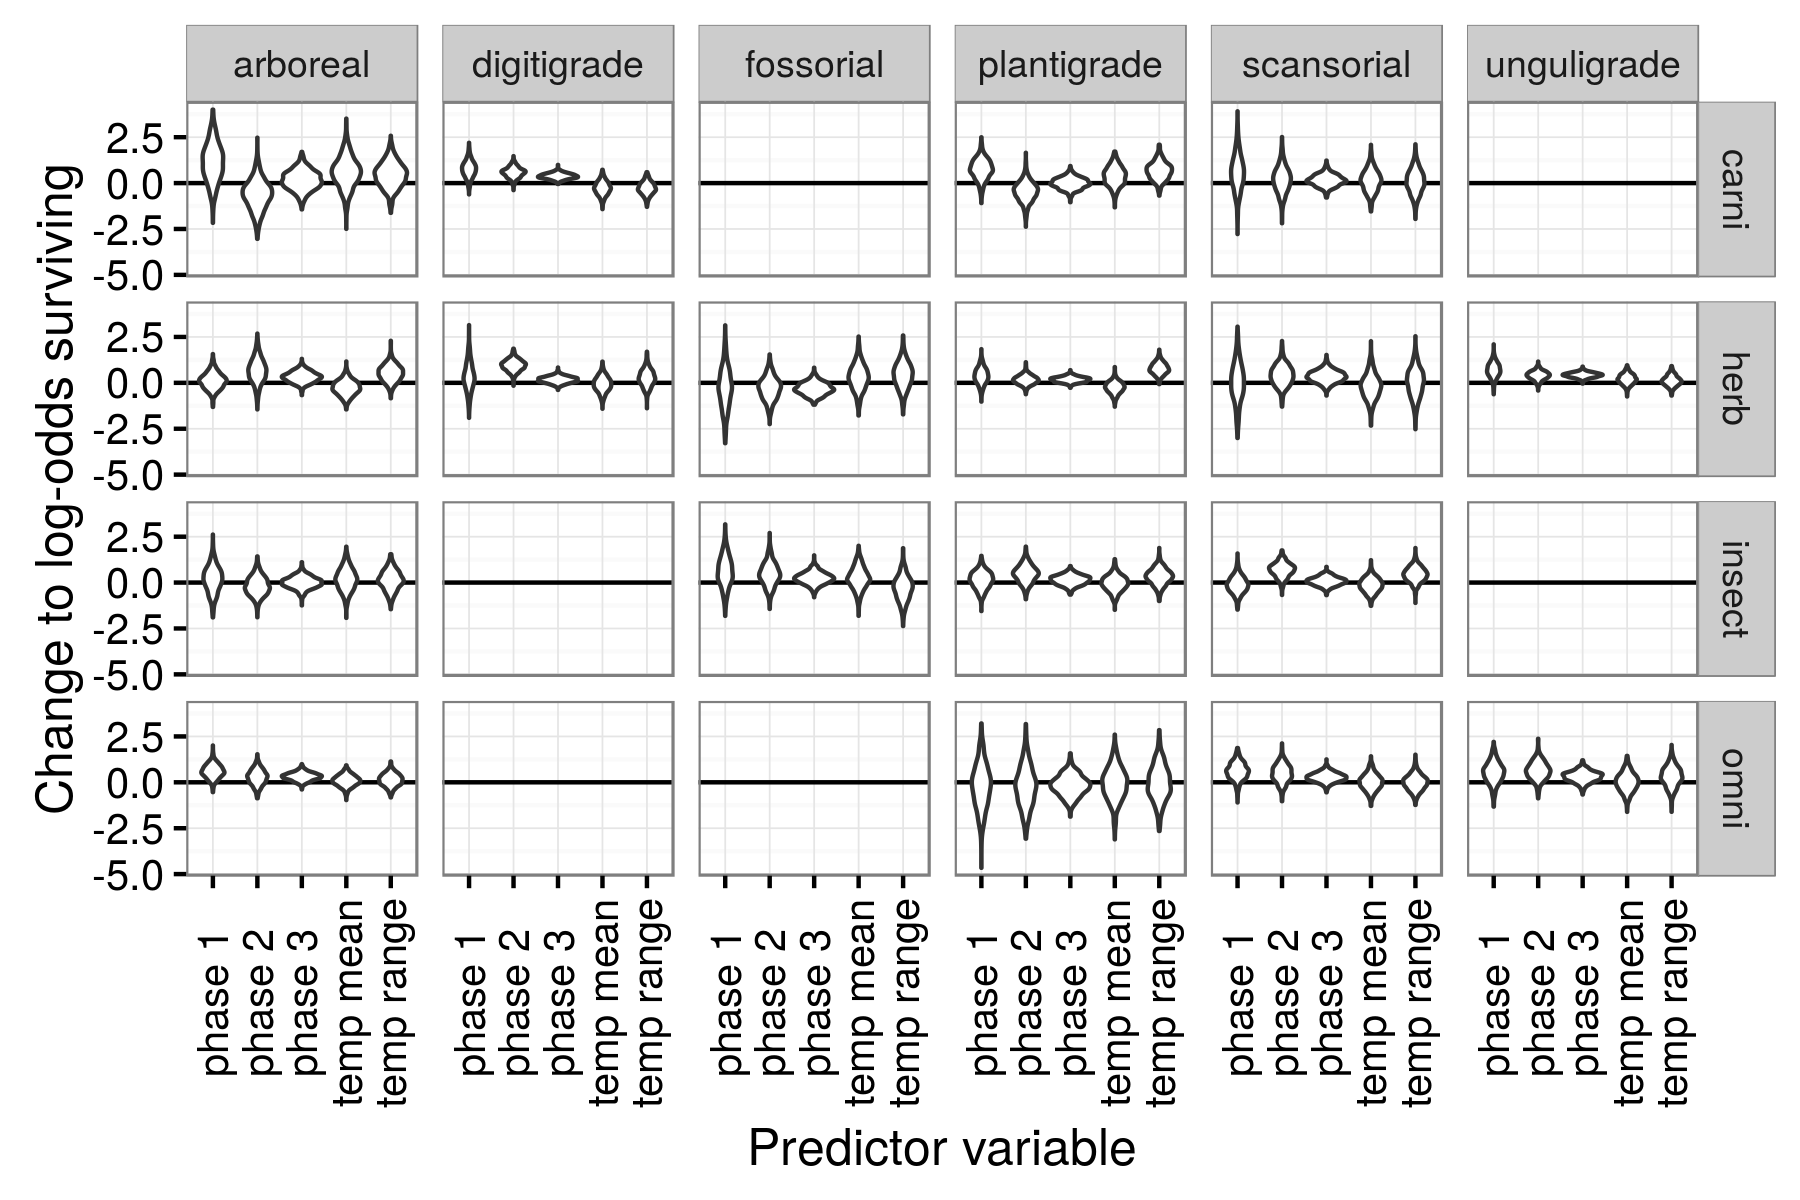
\includegraphics[width=\textwidth,height=0.5\textheight,keepaspectratio=true]{figure/group_on_survival_bd}
  \caption[Effects of group-level covariates on log-odds of ecotype survival as estimated from the the birth-death model]{Estimated effects of the group-level covariates describing environmental context on log-odds of species survlval. These estimates are from the birth-death model.}
  \label{fig:group_surv_bd}
\end{figure}





\subsection*{Analysis of diversity}

All of the following analyses of diversification and macroevolutionary rates has been done using only the birth-death model; this is because of the models better posterior predictive check performance (Fig. \ref{fig:ppc_pure_presence}, and \ref{fig:ppc_birth_death}). 


The general pattern of total estimated North American mammal diversity for the Cenozoic is ``stable'' in that mean standing diversity does not fluctuate wildly and rapidly over the Cenozoic (Fig. \ref{fig:diversity_est}). In broad strokes, the first 15 or so million years of the Cenozoic are characterized by a gradual decline in standing diversity until approximately 45-50 million years ago (early-middle Eocene). Following this decline, standing diversity is broadly constant from 45 to 18 Mya (early Miocene). After this, there is a rapid spike in diversity followed by a slight decline in diversity up to the Modern. This characterization of the estimated diversity history is knowingly broad strokes and diversity time series is not without variation and vagaries.

When viewed through the lens of diversification rate, some of the structure behind the estimated diversity history begins to take shape (Fig. \ref{fig:diversity_rate}). For most of the Cenozoic, the diversification rate hovers around zero, punctuated by both positive and negative spikes. The largest spike in diversification rate is at 16 Mya, which is early Oligocene (Fig. \ref{fig:diversity_rate}). Other notable increases in diversification rate occur at 54, 44, 36, 26, and 20 Mya; other possible increases in diversification rate are less certain (e.g. 8 Mya). Notable decreases in diversification rate occur at 52, 48, 42, 32, 14, 10, and 6 Mya. 

The comparison between per capita origination and extinction rate estimates reveals how diversification rate is formed (Fig. \ref{fig:origin_rate}, \ref{fig:extinct_rate}). As expected given previous inspection of origination and survival probabilities, diversification rate seems most driven by changes in origination rate as opposed to extinction rate. 
Extinction rate, on the other hand, demonstrates an almost saw-toothed pattern around a constant mean.

Now ask what origin or extinct are doing at the important time points indicated above.

Increases in diversification rate at 54, 44, 36, 26, 20, 16

Decreases in diversification rate at 52, 48, 42, 32, 14, 10, 6


\begin{figure}[ht]
  \begin{subfigure}[b]{0.45\textwidth}
    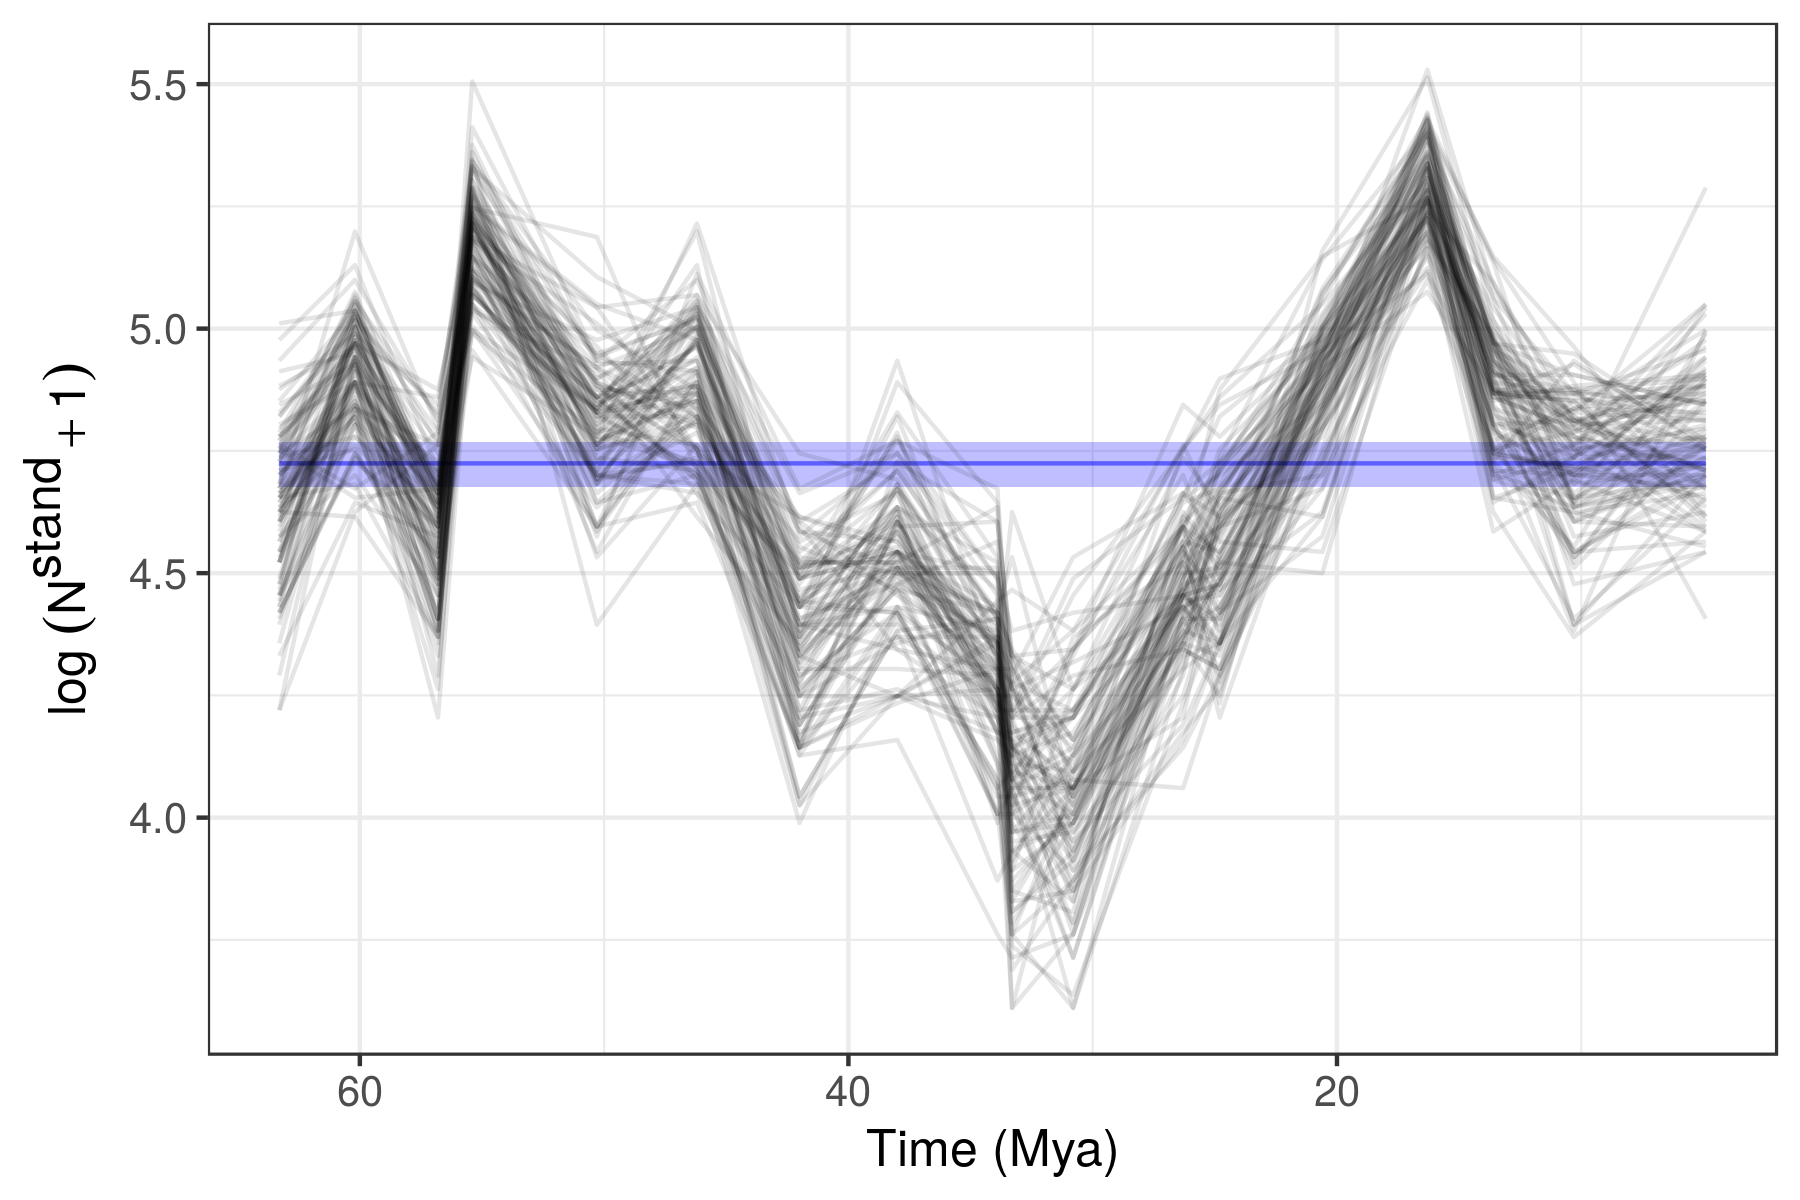
\includegraphics[width=\textwidth,height=0.5\textheight,keepaspectratio=true]{figure/log_diversity}
    \caption{Log diversity}
    \label{fig:diversity_est}
  \end{subfigure}
  \begin{subfigure}[b]{0.45\textwidth}
    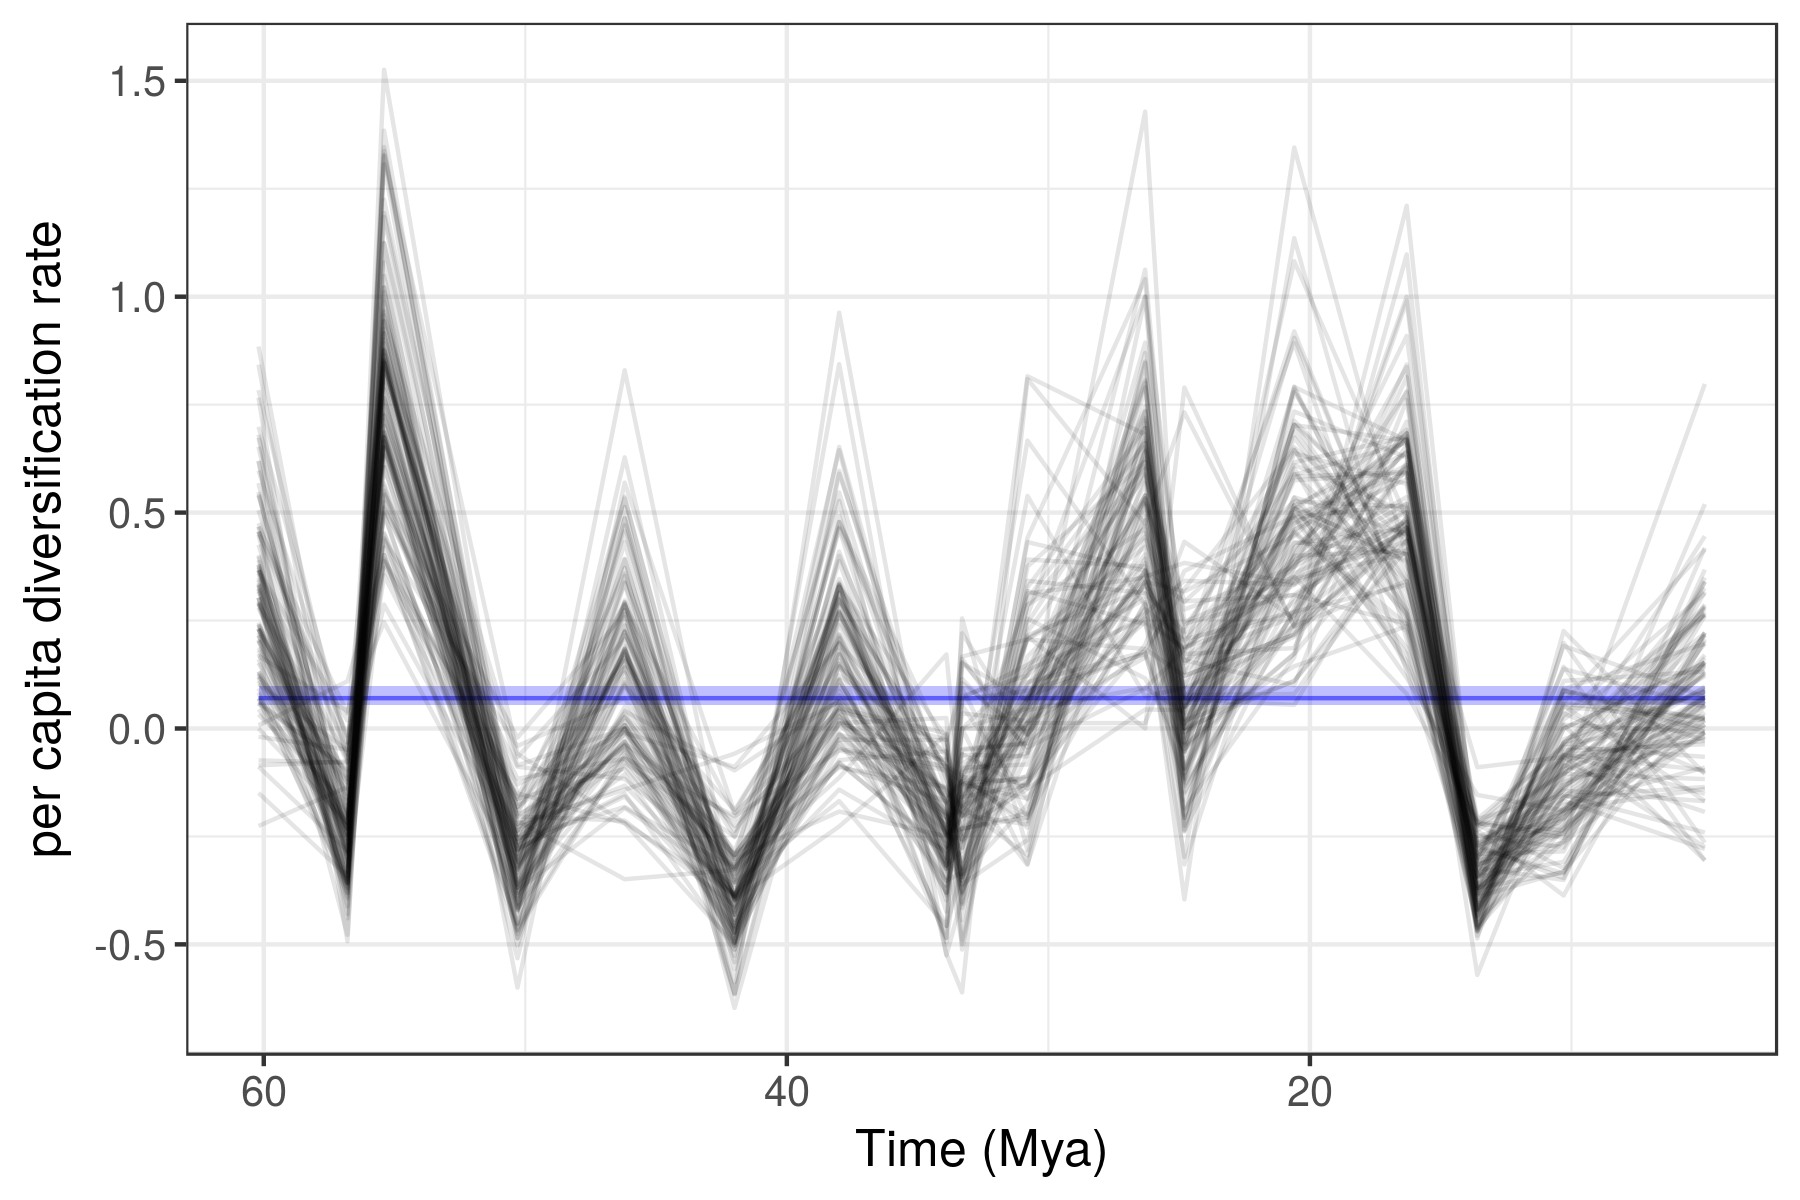
\includegraphics[width=\textwidth,height=0.5\textheight,keepaspectratio=true]{figure/div_rate}
    \caption{Diversification rate}
    \label{fig:diversity_rate}
  \end{subfigure}

  \begin{subfigure}[b]{0.45\textwidth}
    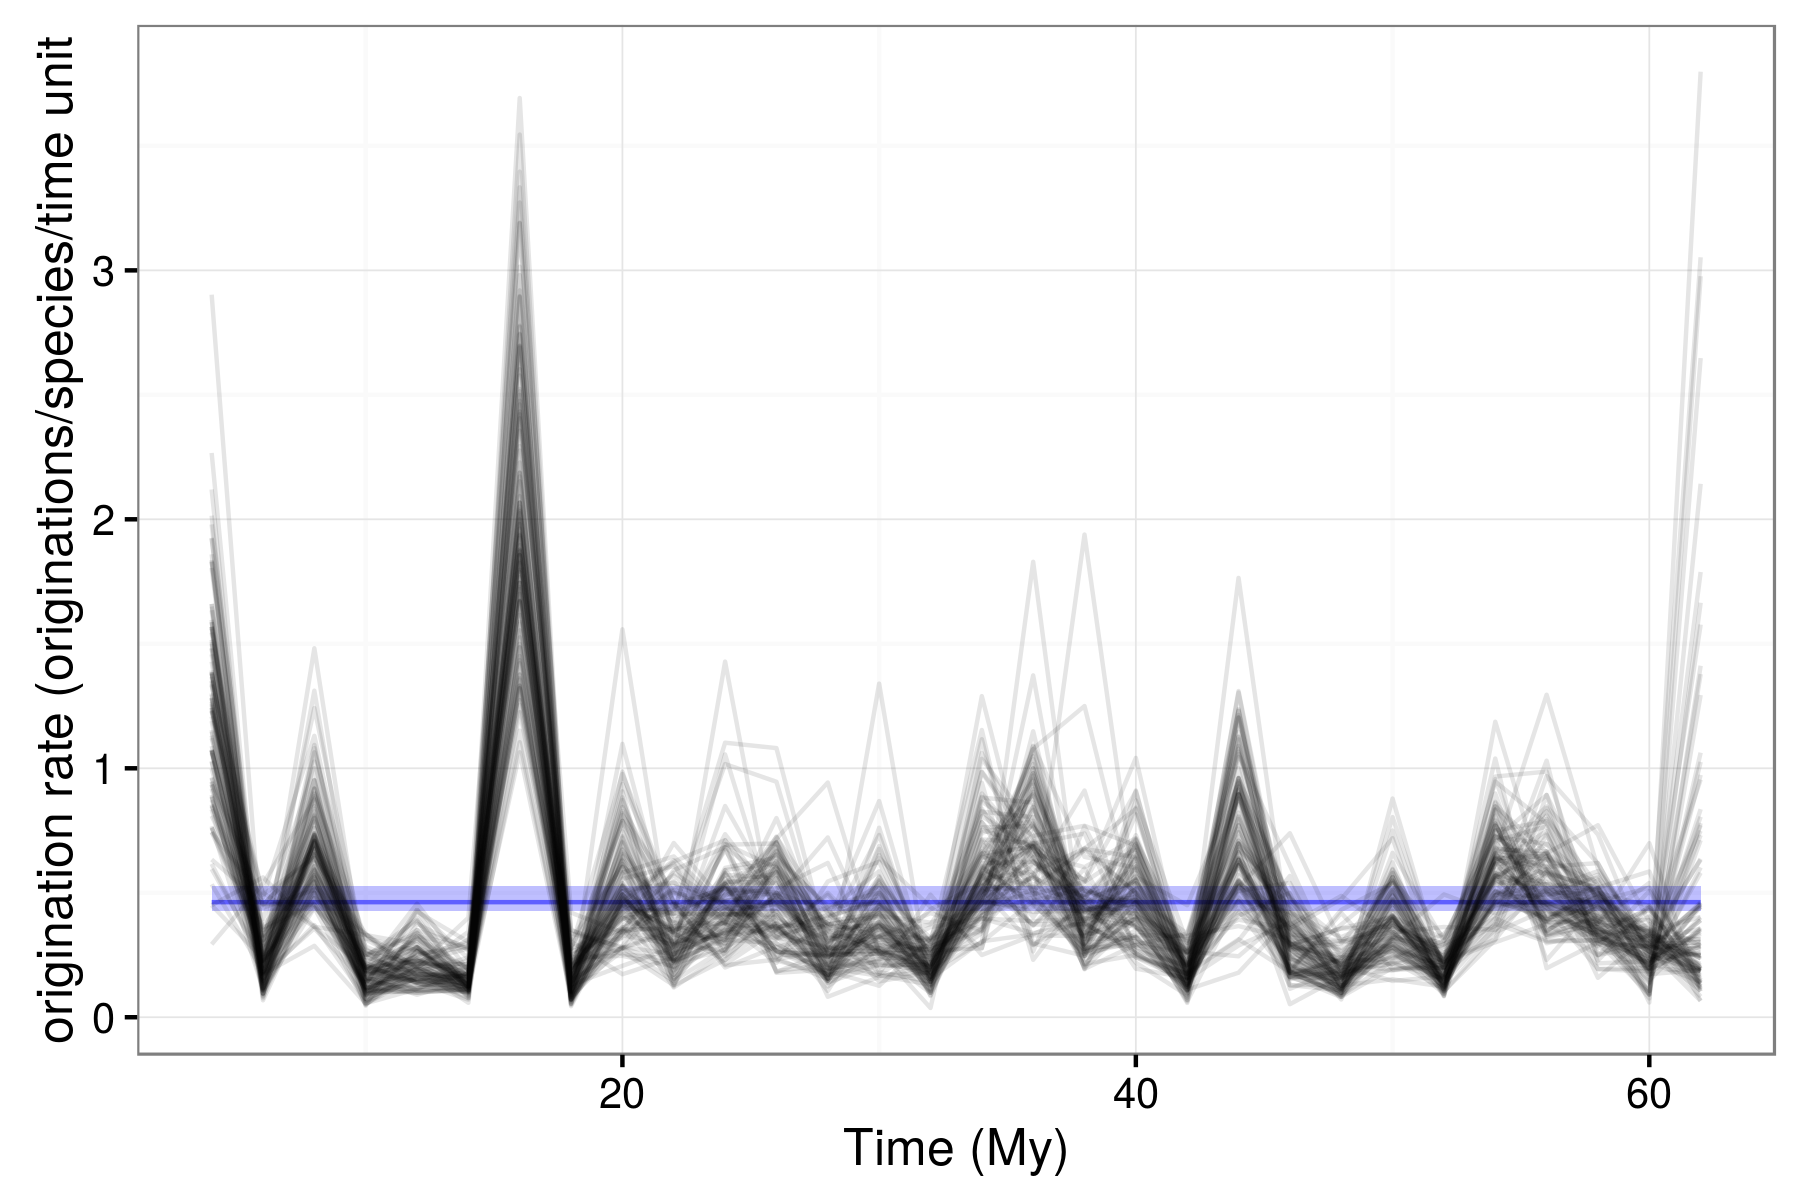
\includegraphics[width=\textwidth,height=0.5\textheight,keepaspectratio=true]{figure/orig_rate}
    \caption{Origination rate}
    \label{fig:origin_rate}
  \end{subfigure}
  \begin{subfigure}[b]{0.45\textwidth}
    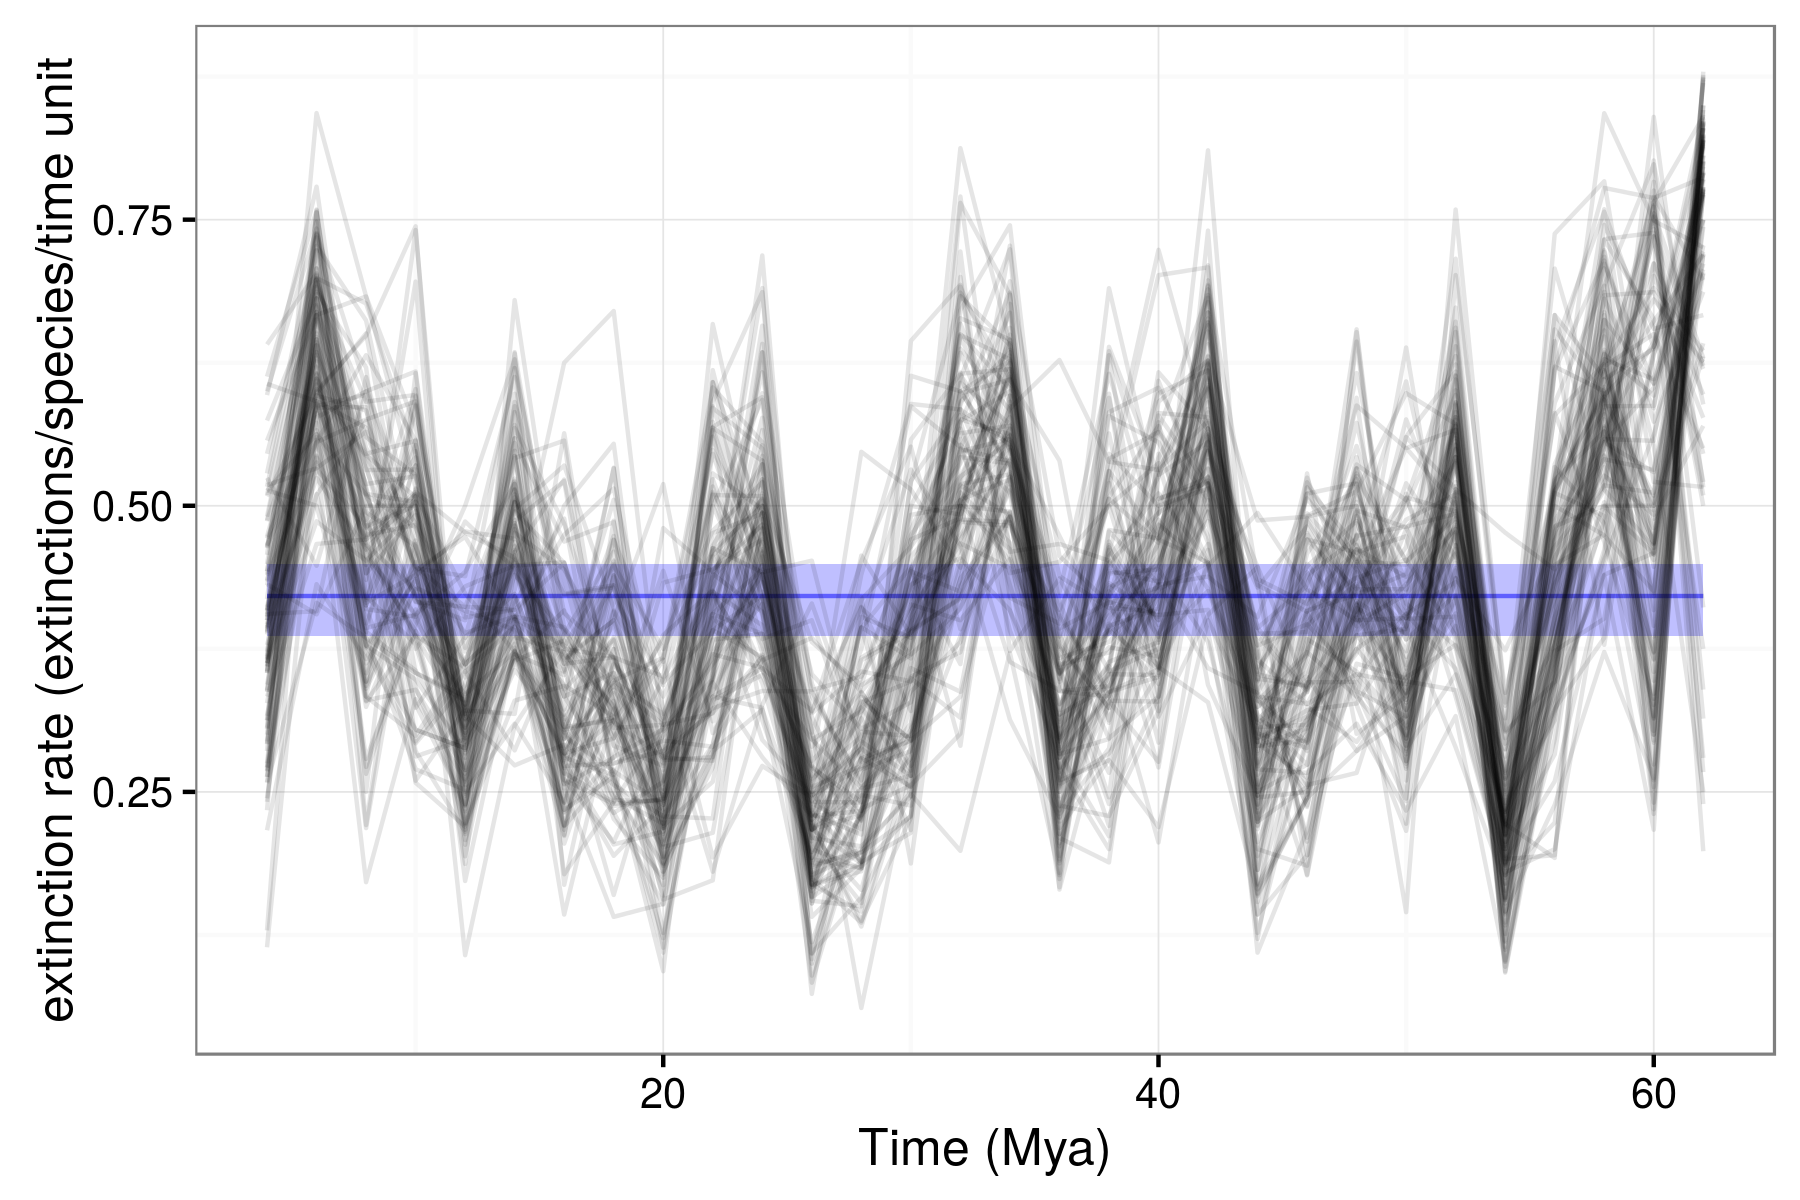
\includegraphics[width=\textwidth,height=0.5\textheight,keepaspectratio=true]{figure/death_rate}
    \caption{Extinction rate}
    \label{fig:extinct_rate}
  \end{subfigure}
  \caption[Estimated mammal log-diversity and macroevolutionary rates for the Cenozoic]{Posterior estimates of the time series of Cenozoic North American mammal diversity and it's characteristic macroevolutionary rates; all estimates are from the birth-death model and 100 posterior draws are plotted to indicate the uncertainty in these estimates. The dramatic differences between diversity estimates at the first and second time points and the penultimate and last time points in this series are caused by well known edge effects in discrete-time birth-death models caused by \(p_{\_, t = 1}\) and \(p_{\_, t = T}\) being partially unidentifiable \citep{Royle2008}; the hierarchical modeling strategy used here helps mitigate these effects but they are still present \citep{Gelman2013d,Royle2008}. Diversification rate is in units of species gained per species present per time unit (2 My), origination rate is in units of species originating per species present per time unit, and extinction rate is in units of species becoming extinct per species present per time unit.}
  \label{fig:macro_values}
\end{figure}



Diversity partitioned by ecotype reveals a lot of the complexity behind the pattern of mammal diversity for the Cenozoic (Fig. \ref{fig:ecotype_diversity}). 

Arboreal ecotypes obtain peak diversity early in the Cenozoic and then decline for the rest of the time series, becoming increasingly rare or absent as diversity approaches the Modern (Fig. \ref{fig:ecotype_diversity}). Arboreal herbivores and omnivores obtain peak diversity at the beginning of the Cenozoic then go into decline while still possibly remaining a part of the species pool, while arboreal carnivores and insectivores obtain peak diversity 52-50 Mya and then quickly decline and become extremely rare or absent from the species pool.

The diversity of both digitigrade and unguligrade herbivores increase over the Cenozoic (Fig. \ref{fig:ecotype_diversity}). In contrast, plantigrade herbivore diversity does not have a single, broad-strokes pattern; instead, diversity increases, decreases, and may have then increased till the Modern. Contrastingly, fossorial and scansorial herbivores demonstrate a much flatter history of diversity, with a slight increase in diversity that over time is more pronounced among fossorial taxa than scansorial taxa.

Digitigrade carnivores have a multi-modal diversity history, with peaks 54-52 and 12-10 Mya (Fig.\ref{fig:ecotype_diversity}). Between these two peaks digitigrade carnivore diversity dips below average diversity following the first peak and then grows slowly until the second peak. Plantigrade carnivores obtain peak diversity in the early Cenozoic and then maintain a relatively stable diversity until another peak at the end of the Cenozoic.

There are some broad similarities in diversity histories of insectivorous and omnivorous taxa. The diversity histories of arbreal, plantigrade, and scansorial insectivorous taxa all demonstrate a decreasing pattern with time, while fossorial insectivores have a flat diversity history with a rapid peak approximately 10 Mya (Fig. \ref{fig:ecotype_diversity}). Arboreal and scansorial omnivores decrease in diversity from their initial peaks early in the Cenozoic, and plantigrade omnivores have a generally flat diversity history with a sudden peak in diversity late in the Cenozoic (Fig. \ref{fig:ecotype_diversity}). Unguligrade omnivores also demonstrate a possible decrease in diversity over the Cenozoic, but not as clearly as arboreal and scansorial omnivores.

Many of the estimated ecotype specific diversity histories share a similar increases in diversity to one degree or another at the late Cenozoic 16-14 Mya (Fig. \ref{fig:ecotype_diversity}); these increases are either sustained or temporary: digitigrade carnivores, plantigrade carnivores, scansorial carnivores, unguligrade herbivores, fossorial insectivores, and plantigrade omnivores.

\begin{figure}[ht]
  \centering
  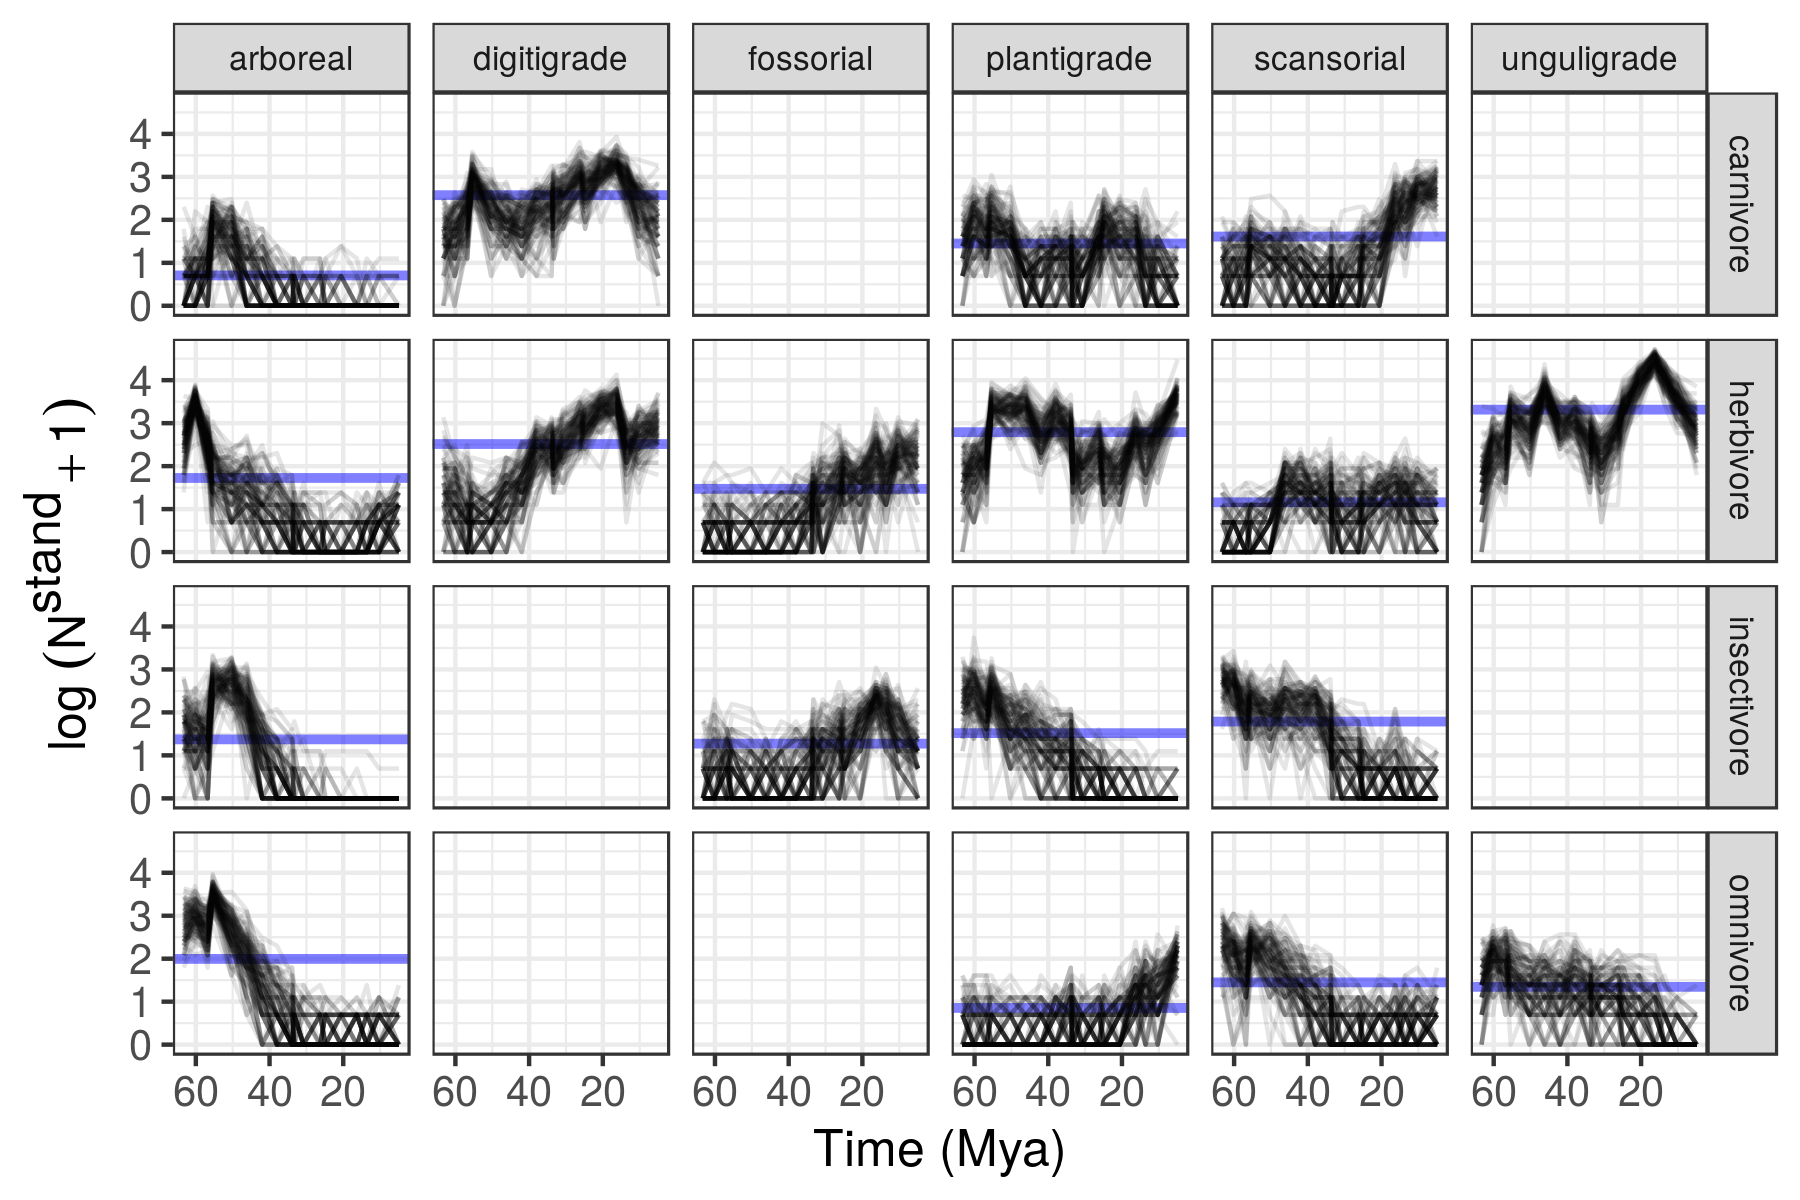
\includegraphics[width=\textwidth,height=0.5\textheight,keepaspectratio=true]{figure/ecotype_diversity}
  \caption[Estimated mammal ecotype log-diversity for the Cenozoic]{Posterior of standing log-diversity of North American mammals by ecotype for the Cenozoic as estimated from the birth-death model; 100 posterior draws are plotted to indicate the uncertainty in these estimates and what is technically plotted is log of diversity plus 1.}
  \label{fig:ecotype_diversity}
\end{figure}



\end{document}
